\UseRawInputEncoding
\documentclass[
paper=A4,        
fontsize=12,        
DIV=11,           
parskip=half,    
headsepline,   
numbers=noenddot  
]{scrartcl}					% Dokument Grundeinstellungen
%===============================================================================
% DOCUMENT CLASS AND ENCODING
%===============================================================================
% Document class is defined in main .tex file

% Character encoding and language settings
\usepackage[utf8]{inputenc}        % UTF-8 input encoding
\usepackage[T1]{fontenc}           % T1 font encoding for better hyphenation
\usepackage[ngerman]{babel}        % German language support

%===============================================================================
% FONTS AND TYPOGRAPHY
%===============================================================================

% Option 1: Modern and clean (RECOMMENDED)
% \usepackage{libertine}             % Linux Libertine for body text
% \usepackage[libertine]{newtxmath}  % Matching math font
% \usepackage[scaled=0.9]{FiraMono} % Fira Mono for code (modern, readable)

% Option 2: Classic technical documentation
\usepackage[charter]{mathdesign} % Matching math
\usepackage[scaled=0.85]{beramono} % Bera Mono for code

% Option 3: Contemporary sans-serif
% \usepackage[default]{sourcesanspro} % Source Sans Pro
% \usepackage[scaled=0.9]{sourcecodepro} % Source Code Pro

% Typography settings
\usepackage{microtype}             % Improved typography
\usepackage[onehalfspacing]{setspace} % Line spacing
\setstretch{1.15}                  % Fine-tune line spacing
\usepackage[babel,german=guillemets]{csquotes}

%===============================================================================
% PAGE LAYOUT
%===============================================================================
\usepackage[
    left=2.5cm,
    right=2.5cm,
    top=2.5cm,
    bottom=2.5cm,
    headheight=18pt,               % Prevents warnings
    footskip=1.5cm
]{geometry}

%===============================================================================
% COLORS
%===============================================================================
\usepackage[dvipsnames,svgnames,x11names]{xcolor}
% Define project-specific colors
\definecolor{codegreen}{rgb}{0,0.6,0}
\definecolor{codegray}{rgb}{0.5,0.5,0.5}
\definecolor{codepurple}{rgb}{0.58,0,0.82}
\definecolor{backcolour}{rgb}{0.95,0.95,0.92}
\definecolor{accentblue}{HTML}{0066CC}  % For headings/links

%===============================================================================
% MATHEMATICS AND ALGORITHMS
%===============================================================================
\usepackage{amsmath}
% \usepackage{amsfonts}  % Disabled - conflicts with mathdesign
% \usepackage{amssymb}   % Disabled - conflicts with mathdesign
\usepackage{siunitx}               % SI units
\usepackage{algorithm}
\usepackage{algpseudocode}

%===============================================================================
% CODE LISTINGS
%===============================================================================
\usepackage{listings}
\lstset{
    % Basic settings
    basicstyle=\ttfamily\footnotesize,
    breaklines=true,
    breakatwhitespace=true,
    % Frame and numbering
    frame=single,
    framesep=5pt,
    framexleftmargin=5pt,
    numbers=left,
    numberstyle=\tiny\color{codegray},
    numbersep=10pt,
    % Syntax highlighting
    commentstyle=\color{codegreen}\itshape,
    keywordstyle=\color{blue}\bfseries,
    stringstyle=\color{codepurple},
    % Background
    backgroundcolor=\color{backcolour},
    % Spacing
    aboveskip=15pt,
    belowskip=10pt,
    % Other
    showstringspaces=false,
    captionpos=b,
    % German umlauts support
    literate={ä}{{\"a}}1 {ö}{{\"o}}1 {ü}{{\"u}}1 
             {Ä}{{\"A}}1 {Ö}{{\"O}}1 {Ü}{{\"U}}1 
             {ß}{{\ss}}1
}

%===============================================================================
% GRAPHICS AND FIGURES
%===============================================================================
% \usepackage[final]{graphicx}  % final mode ignores missing images more gracefully - loaded in main document
\usepackage{adjustbox}             % Advanced image sizing and overflow protection
\usepackage{placeins}              % FloatBarrier for controlling figure placement
\usepackage{float}                 % For [H] positioning
\usepackage{subcaption}            % Subfigures
\usepackage{pdfpages}              % Include PDF pages
\usepackage{background}

% Configure graphics path
\graphicspath{{images/}{figures/}{diagrams/}}

% Caption setup
\usepackage[
    font=small,
    labelfont=bf,
    format=plain,
    justification=justified,
    singlelinecheck=false
]{caption}
\captionsetup[subfigure]{labelformat=empty}

% Background setup
\backgroundsetup{contents={}}

\newcommand{\tocgroup}[1]{%
    \addtocontents{toc}{\protect\vspace{3.5em}}%
    \addtocontents{toc}{\protect\noindent\protect\rule{\textwidth}{0.2pt}}%
    \addtocontents{toc}{\protect\vspace{0.1em}}%
    \addtocontents{toc}{\protect\centerline{\protect\parbox{0.8\textwidth}
    {\protect\centering\textbf{#1}}}}%
    \addtocontents{toc}{\protect\vspace{0.3em}}%
}

%===============================================================================
% TABLES
%===============================================================================
\usepackage{tabularx}
\usepackage{booktabs}              % Professional tables
\usepackage{longtable}             % Multi-page tables
\usepackage{array}                 % Enhanced arrays/tables

%===============================================================================
% HEADERS AND FOOTERS
%===============================================================================
\usepackage[automark]{scrlayer-scrpage}
\clearpairofpagestyles
\pagestyle{scrheadings}
\ihead{Lauterbach, Marty}
\chead{}
\ohead{\today}
\ifoot{}
\cfoot{}
\ofoot[{\thepage\ von \pageref*{LastPage}}]{\thepage\ von \pageref*{LastPage}}

%===============================================================================
% BIBLIOGRAPHY
%===============================================================================
% \usepackage[
%     backend=biber,
%     style=numeric,
%     sorting=none,
%     maxbibnames=99
% ]{biblatex}

%===============================================================================
% HYPERLINKS AND PDF METADATA
%===============================================================================
\usepackage{lastpage}
\usepackage[
    plainpages=false,
    pdfusetitle,
    bookmarks=true,
    bookmarksnumbered=true,
    bookmarksopen=true,
    breaklinks=true
]{hyperref}

\hypersetup{
    pdftitle={M.A.S.K. - Machine-Learning Assisted Skeleton Kinect Tracking},
    pdfauthor={Marty Lauterbach},
    pdfsubject={MKI-Projekt Dokumentation - Interdisziplinäre Motion-Capture-Lösung},
    pdfkeywords={Motion Capture, MediaPipe, Kinect, TouchDesigner, Performance Art},
    pdfproducer={pdfLaTeX},
    colorlinks=true,
    linkcolor=black,
    citecolor=accentblue,
    urlcolor=accentblue,
    pdfdisplaydoctitle=true
}

\usepackage{svg}
% Configure SVG package for better compatibility
\svgsetup{
    inkscapeexe={inkscape},
    inkscapearea=page,
    inkscapelatex=false
}

%===============================================================================
% MISCELLANEOUS
%===============================================================================
% \usepackage[normalem]{ulem}        % Underline/strikethrough
\setcounter{tocdepth}{2}           % TOC depth (sections and subsections)

% Compact ToC formatting to fit in 2 pages
\usepackage{tocloft}
\usepackage{color}
\renewcommand{\cftsecleader}{\cftdotfill{\cftdotsep}}
\setlength{\cftbeforesecskip}{0.2em}
\setlength{\cftbeforesubsecskip}{0.1em}

\rmfamily                          % Roman family default

%===============================================================================
% CUSTOM COMMANDS (Optional)
%===============================================================================
\newcommand{\mask}{\textsc{M.A.S.K.}\xspace}
\newcommand{\code}[1]{\texttt{#1}}
\newcommand{\file}[1]{\texttt{#1}}
\begin{document}
	
	\hypersetup{pageanchor=false}
	
		\begin{titlepage}
	% Kopfzeile enthält das INFLogo als Bild
	\begin{figure}
		\begin{flushright}
			
\includegraphics[scale=0.75]{images/INFLogo.png}
		\end{flushright}
	\end{figure}

	{\centering
		
		\vspace{3.5cm}
		{\Large  MKI-Projekt SoSe 2025}\\
		\vspace{1cm}
		{\LARGE{\textbf{M.A.S.K.}} \\
        \vspace{0.5cm}
        \textbf{\color{Goldenrod}M}achine-Learning \textbf{\color{Goldenrod}A}ssisted \\
        \textbf{\color{Goldenrod}S}keleton \textbf{\color{Goldenrod}K}inect Tracking \\
        }
        
		\vspace{5cm}
		Marty Lauterbach\\
		\href{mailto:martin.lauterbach@student.reutlingen-university.de}{martin.lauterbach@student.reutlingen-university.de}\\
        \vspace{0.2cm}
        
		Akademische Aufsicht: Prof. Dipl.-Ing. Anja Hartmann \\
		
		\vspace{0.2cm}
		{\small Abgabedatum: \today}\\

        \vspace{2.5cm}
        \begin{center}
        In Kooperation mit\\
        \vspace{0.3cm}
        
\includegraphics[height=1.2cm]{images/FAWB.pdf}
        \end{center}
	}
	
	% Fußzeile enthält die Anschrift und das Logo der Reutlingen University
	\backgroundsetup{
		scale=1,
		color=black,
		opacity=1,
		angle=0,
		position=current page.south,
		vshift=60pt,
		hshift=-200pt,
		contents={
			\begin{minipage}{.18\textwidth}
				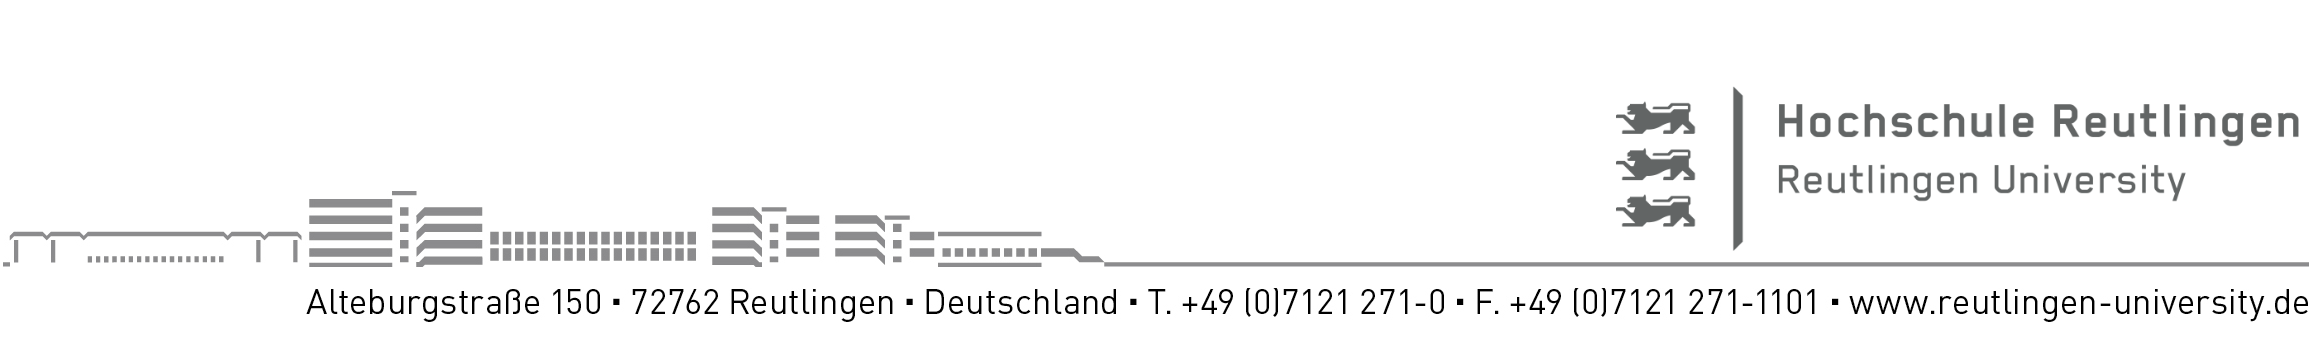
\includegraphics[width=1000pt,height=70pt,keepaspectratio]{images/FHRTFooter.png}
			\end{minipage}
		}
	}
\end{titlepage}	
		
 	\newpage
    \singlespacing
    
    % Kurze Zusammenfassung nach der Titelseite
    \section*{Zusammenfassung}
    M.A.S.K. (Machine-Learning Assisted Skeleton Kinect Tracking) ist ein kostengünstiges Motion-Capture-System, entwickelt für die cinematographische Tanzproduktion \textit{Echoes of the Mind}. Das System kombiniert Kinect V2 Hardware mit MediaPipe-Software und TouchDesigner-Integration für Echtzeitvisualisierungen basierend auf Performerbewegungen.
    
    Die zentrale Innovation liegt in der Infrarot-Adaptation, die zuverlässiges Tracking unter intensiver Beamerbeleuchtung ermöglicht. Das System wurde erfolgreich in professioneller Studioumgebung validiert und demonstriert die Machbarkeit kostengünstiger Motion-Capture-Lösungen für kreative Anwendungen.
    \addcontentsline{toc}{section}{Zusammenfassung}
    
    \newpage
    
    \tableofcontents
    
    \onehalfspacing
    
    \pagenumbering{arabic}
    
    \newpage
	\hypersetup{pageanchor=true}
	
	\setcounter{page}{1}
	
	\captionsetup[subfigure]{labelformat=empty}

    % HAUPTTEIL - Chronologisch logischer Aufbau
    \tocgroup{Projektüberblick}

    \section{Projektvision und Ergebnisse}\label{sec:vision}
        \subsection*{Dokumentationsstruktur}

Diese Dokumentation folgt einem chronologisch-logischen Aufbau, der den Leser vom \textbf{großen Bild zum Detail} führt:

\begin{itemize}
    \item \textbf{Projektüberblick:} Vision, Kooperationskontext und Machbarkeitsstudie
    \item \textbf{Technische Umsetzung:} Anforderungen, Entwicklungsweg und finale Systemarchitektur  
    \item \textbf{Praxisvalidierung:} Produktionsnachweis in der realen Filmproduktion
    \item \textbf{Erkenntnisse:} Zentrale Learnings und Projektbeiträge
    \item \textbf{Technische Dokumentation:} Code-Repository und Teamkommunikation
\end{itemize}

\subsection*{Projektvision}

M.A.S.K. (Machine-Learning Assisted Skeleton Kinect Tracking) entstand aus einer interdisziplinären Kooperation zwischen der Filmakademie Baden-Württemberg und der Hochschule Reutlingen. Das Projekt entwickelte ein kostengünstiges, robustes Motion-Capture-System für die cinematographische Tanzproduktion \textit{Echoes of the Mind}.

Die zentrale Herausforderung bestand in der Entwicklung eines Tracking-Systems, das unter intensiver Beamerbeleuchtung und bei komplexen Bewegungssequenzen zuverlässig funktioniert. Herkömmliche RGB-basierte Tracking-Verfahren zeigen unter diesen Produktionsbedingungen reduzierte Genauigkeit. Zur Lösung wurde eine spezifische Adaptation entwickelt, die Consumer-Hardware und Open-Source-Software kombiniert.

Die Entwicklung durchlief mehrere iterative Phasen: Ein ursprünglich geplanter Dual-Source-Ansatz wurde zugunsten einer vereinfachten MediaPipe-basierten Lösung modifiziert. Die finale Infrarot-Adaptation entstand aus spezifischen Produktionsanforderungen und bewährte sich unter realen Studiobedingungen.

Das resultierende System basiert auf einer modularen Architektur mit TouchDesigner-Containern, die flexible Integration in bestehende Produktions-Workflows ermöglichen. Die Implementation verarbeitet Kamera-Streams in Echtzeit, extrahiert Skelettdaten über MediaPipe und stellt strukturierte Koordinaten für Visualisierungssysteme bereit. Spezialisierte Python-Skripte ermöglichen die direkte Integration in TouchDesigner für ParticleGPU-Effekte, Zustandsmaschinen und Trigger-Logiken.

Das M.A.S.K.-System wurde erfolgreich in einer professionellen Filmproduktion validiert und demonstriert die Wirksamkeit kostengünstiger Motion-Capture-Lösungen für spezialisierte Anwendungen. Die modulare Systemarchitektur ermöglicht Reproduzierbarkeit und Erweiterung für ähnliche interdisziplinäre Projekte.

Hervorgebracht wurden zusätzlich Schwierigkeiten bei der Verarbeitung von teilweise verdeckten Performern. Wenn die grundlegenden RGB-Daten nicht ausreichend schlüssig für das MediaPipe-Modell waren, folgte das System einen GIGO-Prinzip: Garbage In, Garbage Out. Das System konnte dann keine sinnvollen Skelettdaten mehr extrahieren. Die finale Infrarot-Adaptation ermöglichte es, in Momenten wo der Beamer auf dem Tänzer ein Problem war, auch bei partieller Sichtbarkeit präzisere Tracking-Daten zu generieren.

Die Entwicklung verdeutlicht das Potenzial interdisziplinärer Kooperationen zwischen technischen Hochschulen und Kunsthochschulen für praxisorientierte Lösungsansätze in der Creative Technology.

\textbf{Open Source:} Der vollständige Quellcode, inklusive TouchDesigner-Projekten und Python-Skripten, sowie dem LaTex dieser Dokumentation, ist verfügbar unter:

\texttt{https://github.com/mklemmingen/MASK}

\textbf{Behind-The-Scenes Video:} Visualisierungen, Debug-Overlays und Setup der Infrarot-Pipeline unter: \texttt{TODO LINK EINFÜGEN}         % Ausführliche Projektvision und Dokumentationsstruktur

    \newpage

    \section{Projektkontext und Kooperation}\label{sec:context}
        \input{src/Einführung}              % Stakeholder-Kontext und "Echoes of the Mind"

    \newpage

    \section{Machbarkeitsstudie}\label{sec:feasibility}
        Einschätzung der Machbarkeit des M.A.S.K.-Projekts (Stand: März 2025) unter Anwendung des TELOS-Frameworks nach Hall (2013)\footnote{Hall, J.A. \textit{Accounting Information Systems, 8th Edition}. Brooks/Cole, 2013.}.

\subsection{Technologisch}

\textbf{Technische Realisierbarkeit:}
Das Projekt ist technisch umsetzbar. Die Kernkomponenten TouchDesigner, MediaPipe und Kinect V2 sind etablierte Technologien mit dokumentierter Kompatibilität. Studien wie Babouras et al. (2024)\footnote{Babouras, A., Abdelnour, P., Fevens, T. et al. „Comparing novel smartphone pose estimation frameworks with the Kinect V2 for knee tracking during athletic stress tests." \textit{International Journal of Computer Assisted Radiology and Surgery} 19, 1321–1328 (2024).} bestätigen die Zuverlässigkeit der Kinect V2-MediaPipe-Kombination für bewegungsbasierte Anwendungen.

\textbf{Technologie-Zugang:}
Das interdisziplinäre Team verfügt über die erforderliche Hardware (Kinect V2) und nutzt TouchDesigner 2023.11 in der kostenlosen Bildungsversion. Die Filmakademie Ludwigsburg stellt zusätzliche Studioinfrastruktur bereit.

\textbf{Stakeholder-Akzeptanz:}
Die Technologiewahl wurde gemeinsam mit der Filmakademie getroffen, wodurch hohe Akzeptanz und aktive Unterstützung gewährleistet sind.

\subsection{Economic}

\textbf{Finanzierung:}
Das Projekt wird im Rahmen des regulären Studiums durchgeführt, ohne externe Finanzierung. Die einzigen Kosten entstehen durch die Kinect V2-Hardware (ca. 90€), die privat beschafft wurde. TouchDesigner und MediaPipe sind kostenfrei verfügbar.

\subsection{Legal}

\textbf{Lizenzrechtliche Aspekte:}
\begin{itemize}
    \item MediaPipe: Apache License 2.0\footnote{\url{https://github.com/google-ai-edge/mediapipe/blob/master/LICENSE}}
    \item Kinect V2 (libfreenect2): Open-Source-Lizenz\footnote{\url{https://zenodo.org/records/50641}}
    \item TouchDesigner: Nicht-kommerzielle Bildungslizenz\footnote{\url{https://derivative.ca/UserGuide/Licensing}}
\end{itemize}

Alle verwendeten Technologien sind für nicht-kommerzielle Bildungsprojekte frei nutzbar.

\subsection{Operational}

\textbf{Implementierungsanforderungen:}
\begin{itemize}
    \item Entwicklung einer synchronisierten Datenfusion zwischen Kinect V2 und MediaPipe
    \item Implementation regelbasierter Trigger für Visualisierungssteuerung
    \item Integration in die bestehende TouchDesigner-Pipeline der Filmakademie
    \item Koordination zwischen beiden Standorten (Reutlingen/Ludwigsburg)
\end{itemize}

\textbf{Projektmanagement:}
Regelmäßige Online-Meetings und punktuelle Präsenztreffen ermöglichen effektive Zusammenarbeit zwischen den Projektteams.

\subsection{Scheduling}

\textbf{Zeitplanung:}
\begin{itemize}
    \item \textbf{Projektlaufzeit:} Januar bis Mai 2025
    \item \textbf{Prototyp-Ziel:} Mitte April 2025
    \item \textbf{Finaler Einsatz:} Filmproduktion Mai 2025
    \item \textbf{Ressourcenallokation:} 2 feste Projekttage pro Woche
\end{itemize}

\textbf{Risikomanagement:}
Der modulare Entwicklungsansatz ermöglicht eine stufenweise Implementierung und reduziert das Risiko von Zeitüberschreitungen. Parallele Studienverpflichtungen wurden durch Workload-Anpassungen in anderen Modulen kompensiert.            % Vorab-Analyse (TELOS-Framework)

    \tocgroup{Technische Umsetzung}

    \newpage

    \section{Anforderungen und Designentscheidungen}\label{sec:requirements}
        \subsection{Änderungsverlauf}
\begin{table}[h]
    \centering
    \begin{tabular}{|c|c|c|p{7cm}|}
        \hline
        \textbf{Version} & \textbf{Datum} & \textbf{Autor} & \textbf{Änderungen} \\ \hline
        1.0 & 27.01.2025 & M. Lauterbach & Initialer Stakeholder-Kontakt und Grundanforderungen definiert \\ \hline
        1.1 & 22.02.2025 & M. Lauterbach & TELOS-Machbarkeitsstudie erstellt \\ \hline
        1.2 & 03.03.2025 & M. Lauterbach & Dokumentationsstruktur etabliert \\ \hline
        1.3 & 05.03.2025 & M. Lauterbach & Sprachliche Überarbeitung und Korrekturen \\ \hline
        1.4 & 10.03.2025 & M. Lauterbach & Choreographie-spezifische Anforderungen (FA-07 bis FA-12) integriert \\ \hline
        1.5 & 30.03.2025 & M. Lauterbach & Visual-Design-Anforderungen nach Stakeholder-Feedback erweitert \\ \hline
        1.6 & 17.04.2025 & M. Lauterbach & Restriktive Präzisierung der Anforderungen basierend auf finalen Visual-Spezifikationen für Systemintegration \\ \hline
    \end{tabular}
    \caption{Dokumentations-Changelog}
    \label{tab:changelog}
\end{table}

\subsubsection{Technische Infrastruktur der Filmakademie}
\begin{itemize}
    \item \textbf{Hardware:} NVIDIA RTX 3080, AMD Ryzen 9750
    \item \textbf{Software:} TouchDesigner 2023.11
    \item \textbf{Tracking:} Kinect V2 mit RGB- und Tiefensensor
    \item \textbf{Studiodimensionen:} 383 m² (21m × 15m)
\end{itemize}

\subsection{Funktionale Anforderungen}

\textbf{Kern-Tracking-Funktionalität:}
\begin{itemize}
    \item \textbf{FA-01:} Einfachpersonen-Erkennung und -Verfolgung im Kinect-Sichtfeld
    \item \textbf{FA-02:} Echtzeit-Verarbeitung der Positionsdaten für regelbasierte Trigger
    \item \textbf{FA-05:} Native TouchDesigner-Integration für Visualisierungssteuerung
    \item \textbf{FA-06:} Modulare Systemarchitektur für iterative Optimierung
\end{itemize}

\textbf{Performance-spezifische Anforderungen:}
\begin{itemize}
    \item \textbf{FA-07:} Boolean-Node-Triggering/Switch-Triggers und Python-basierte Eigenschaftsmanipulation
    \item \textbf{FA-08:} Personen-Eintrittserkennung mit automatischer Aktivierung
    \item \textbf{FA-09:} Selektives Single-Person-Tracking (Kameramann-Ausblendung)
\end{itemize}

\textbf{Projections-Mapping-Funktionalität:}
\begin{itemize}
    \item \textbf{FA-11:} Beamer-Kinect-Kalibrierung für präzise Performer-Ausblendung/Hervorhebung
    \item \textbf{FA-14:} Relative 2D-Positionierung der Visuals zum Performer
\end{itemize}

\textbf{Choreographie-spezifische Visualisierungslogik:}
\begin{itemize}
    \item \textbf{FA-16:} Extremitäten-responsive Blitzeffekte mit radialer Positionierung
    \item \textbf{FA-17:} Hockbewegung-getriggerte Umrandungseffekte bei kreisförmigen Visuals
\end{itemize}            % Was gebaut werden sollte

    \newpage

    \section{Entwicklungsweg}\label{sec:development}
        Die Entwicklung des M.A.S.K.-Systems durchlief eine fundamentale Transformation – von einem komplexen Dual-Source-Ansatz hin zu einer eleganten Single-Pipeline-Lösung. Diese Evolution demonstriert, wie praktische Produktionsanforderungen zu effektiven technischen Lösungen führen können.

\subsection{Phase 1: Initiale Systemkomplexität (Januar - Februar 2025)}

\textbf{Hybrid-Tracking-Architektur:}
Basierend auf Expertenberatung entwickelte ich zunächst ein komplexes Dual-Source-System:

\begin{figure}[htbp]
    \centering
    \adjustbox{max width=0.9\textwidth, max height=0.85\textheight, keepaspectratio}{%
        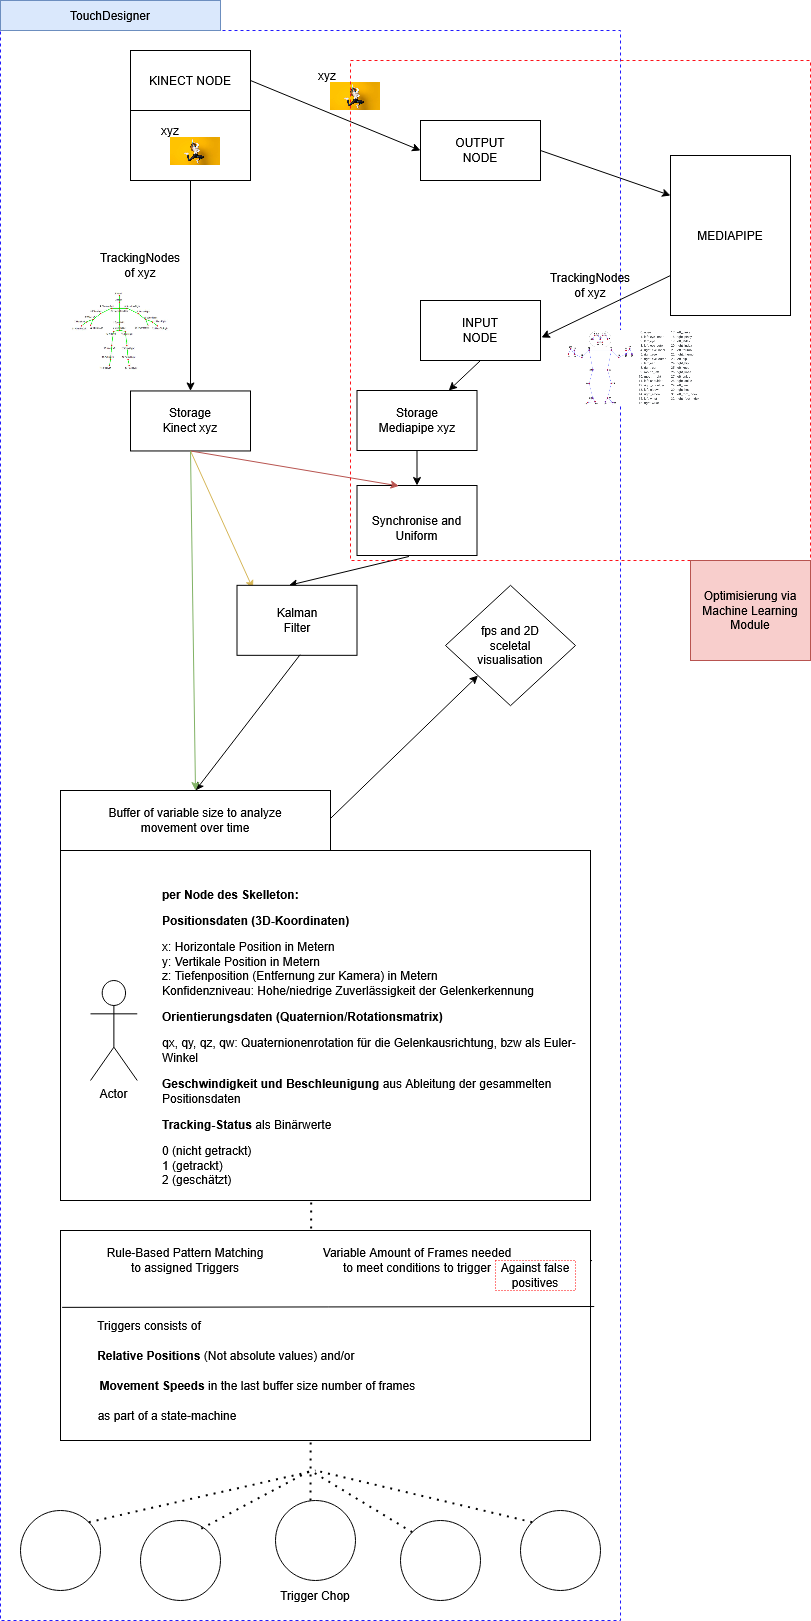
\includegraphics{images/docupictures/MASK.png}%
    }
    \caption{Anfängliches Systemdesin von M.A.S.K. mit Analyse- und Triggerprozess und dem später nach Sprint 2 deprecated Dual-Source-Ansatz}
    \label{fig:mask_architecture}
\end{figure}
\begin{itemize}
    \item \textbf{MediaPipe-Integration:} ML-basierte Pose-Detection über RGB-Stream
    \item \textbf{Native Kinect-Tracking:} Hardware-Skeleton mit Tiefensensor-Daten
    \item \textbf{Kalman-Filter-Fusion:} Synchronisation und Glättung beider Datenquellen
    \item \textbf{Adaptive Fallback-Logik:} Automatische Umschaltung bei Tracking-Verlust
\end{itemize}

\begin{algorithm}[H]
\caption{Ursprüngliche Dual-Source-Verarbeitungsschleife}
\begin{algorithmic}[1]
    \State $\text{kinect\_data} \leftarrow \text{receiveKinectSkeleton()}$
    \State $\text{mediapipe\_data} \leftarrow \text{processRGBStream()}$
    \If{$\text{mediapipe\_data} \neq \text{null} \land \text{kinect\_data} \neq \text{null}$}
        \State $\text{skeleton} \leftarrow \text{fusionProcess}(\text{kinect\_data}, \text{mediapipe\_data})$
    \Else
        \State $\text{skeleton} \leftarrow \text{fallbackToStrongerSource()}$
    \EndIf
    \State $\text{skeleton} \leftarrow \text{applyKalmanFilter}(\text{skeleton})$
    \State \textbf{evaluateTriggers}(\text{skeleton})
\end{algorithmic}
\end{algorithm}

\textbf{Erste Validierung:}
\raggedright Komparative Tests zwischen MediaPipe und Kinect zeigten MediaPipes bessere Robustheit bei partieller Okklusion. Das ML-Modell generierte höhere Confidence-Werte für nicht-sichtbare Körperregionen, was für komplexe Choreographien entscheidend war.

\begin{figure}[htbp]
    \centering
    \adjustbox{max width=0.7\textwidth, max height=0.8\textheight, keepaspectratio}{%
        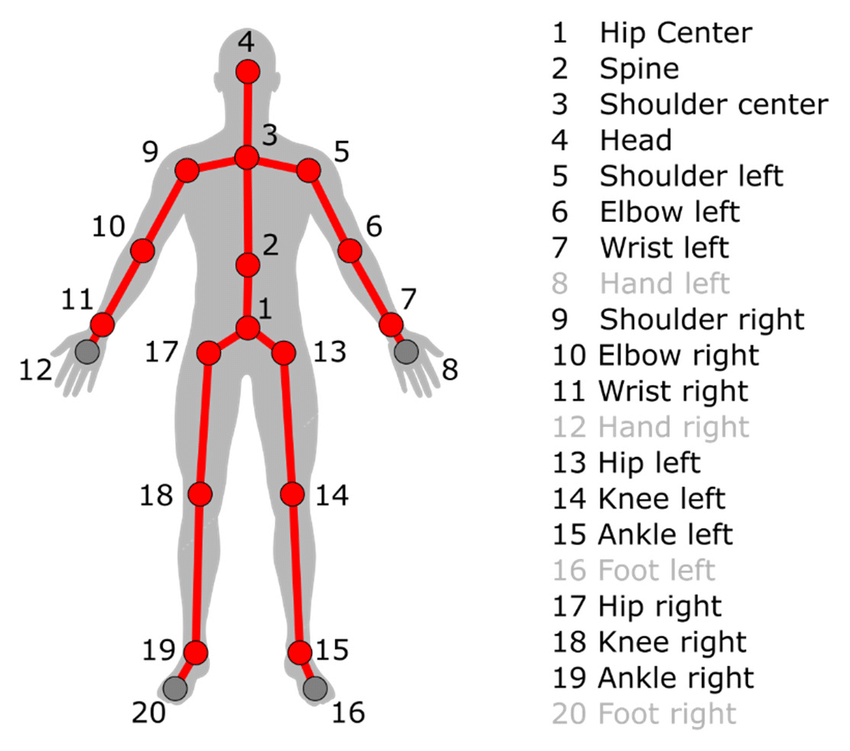
\includegraphics{images/docupictures/kinect_nodes.png}%
    }
    \caption{Kinect V2 Skeleton-Visualisierung mit Node-Nummerierung | Vor Sprint 2 mit MediaPipe Nodes gemischt mit Mapping, später deprecated}
    \label{fig:kinect_nodes}
\end{figure}

\begin{figure}[htbp]
    \centering
    \adjustbox{max width=0.9\textwidth, max height=0.6\textheight, keepaspectratio}{%
        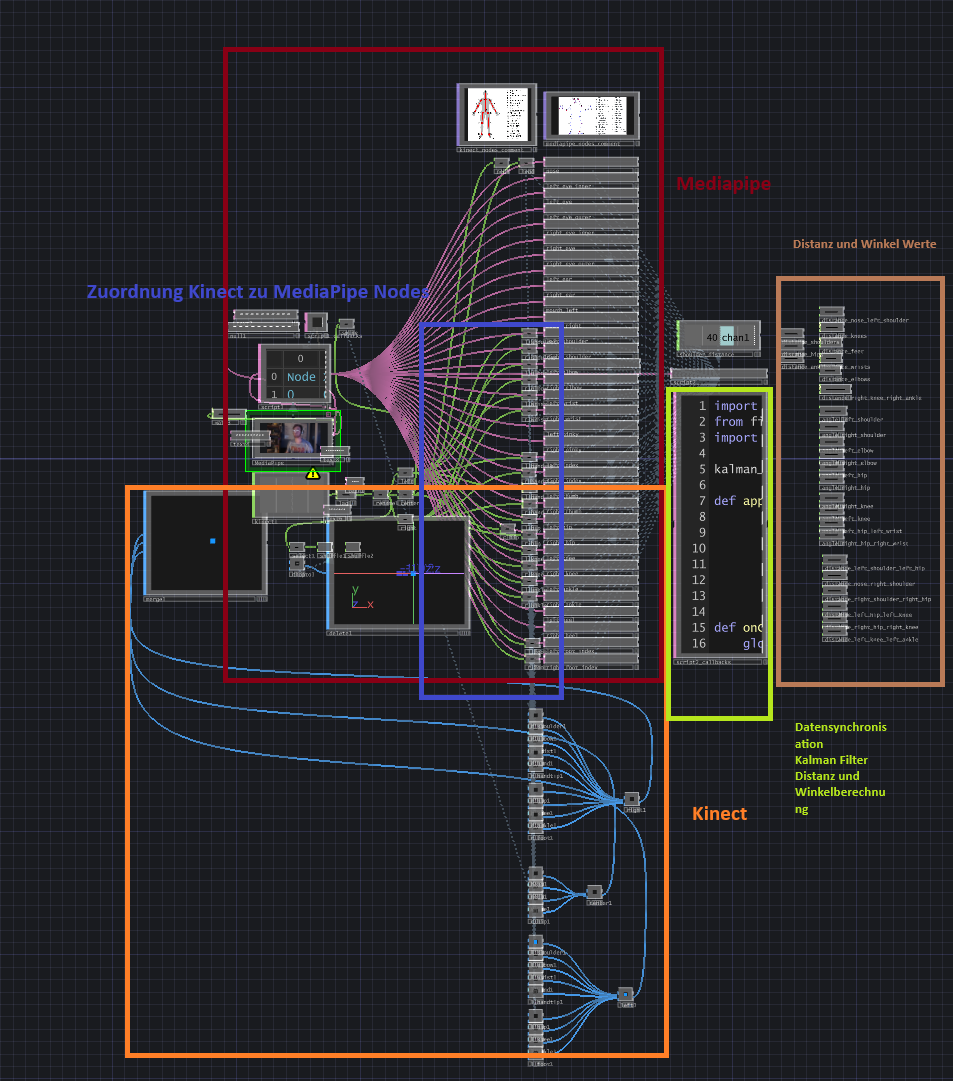
\includegraphics{images/docupictures/KinectMediaPipe_Testing.png}%
    }
    \caption{TouchDesigner Testing-Interface: Unterschied zwischen der Mediapipe Skeleton-Visualisierung (oben, pink) und der Kinect V2 Skeleton-Visualisierung (unten, grün)}
    \label{fig:testing_interface}
\end{figure}

\subsection{Phase 2: Visual Requirements Engineering (März 2025)}

\textbf{Stakeholder-Driven\\Design:}
\raggedright Die intensive Zusammenarbeit mit den Filmakademie-Designerinnen führte zu präzisen Visual-Anforderungen, die über einfache Bewegungstrigger hinausgingen:

\begin{itemize}
    \item \textbf{Adaptive Größenmodulation:} Visuals skalieren basierend auf Performer-Zustand
    \item \textbf{Räumliche Choreographie:} Präzise Beamer-Projektion um Performer herum
    \item \textbf{Emotionale Responsivität:} Visual-Transformation entsprechend choreographischer Intentionen
\end{itemize}

\textbf{Konzeptuelle Visualisierungsansätze:}

\begin{figure}[htbp]
    \centering
    \adjustbox{max width=0.8\textwidth, max height=0.8\textheight, keepaspectratio}{%
        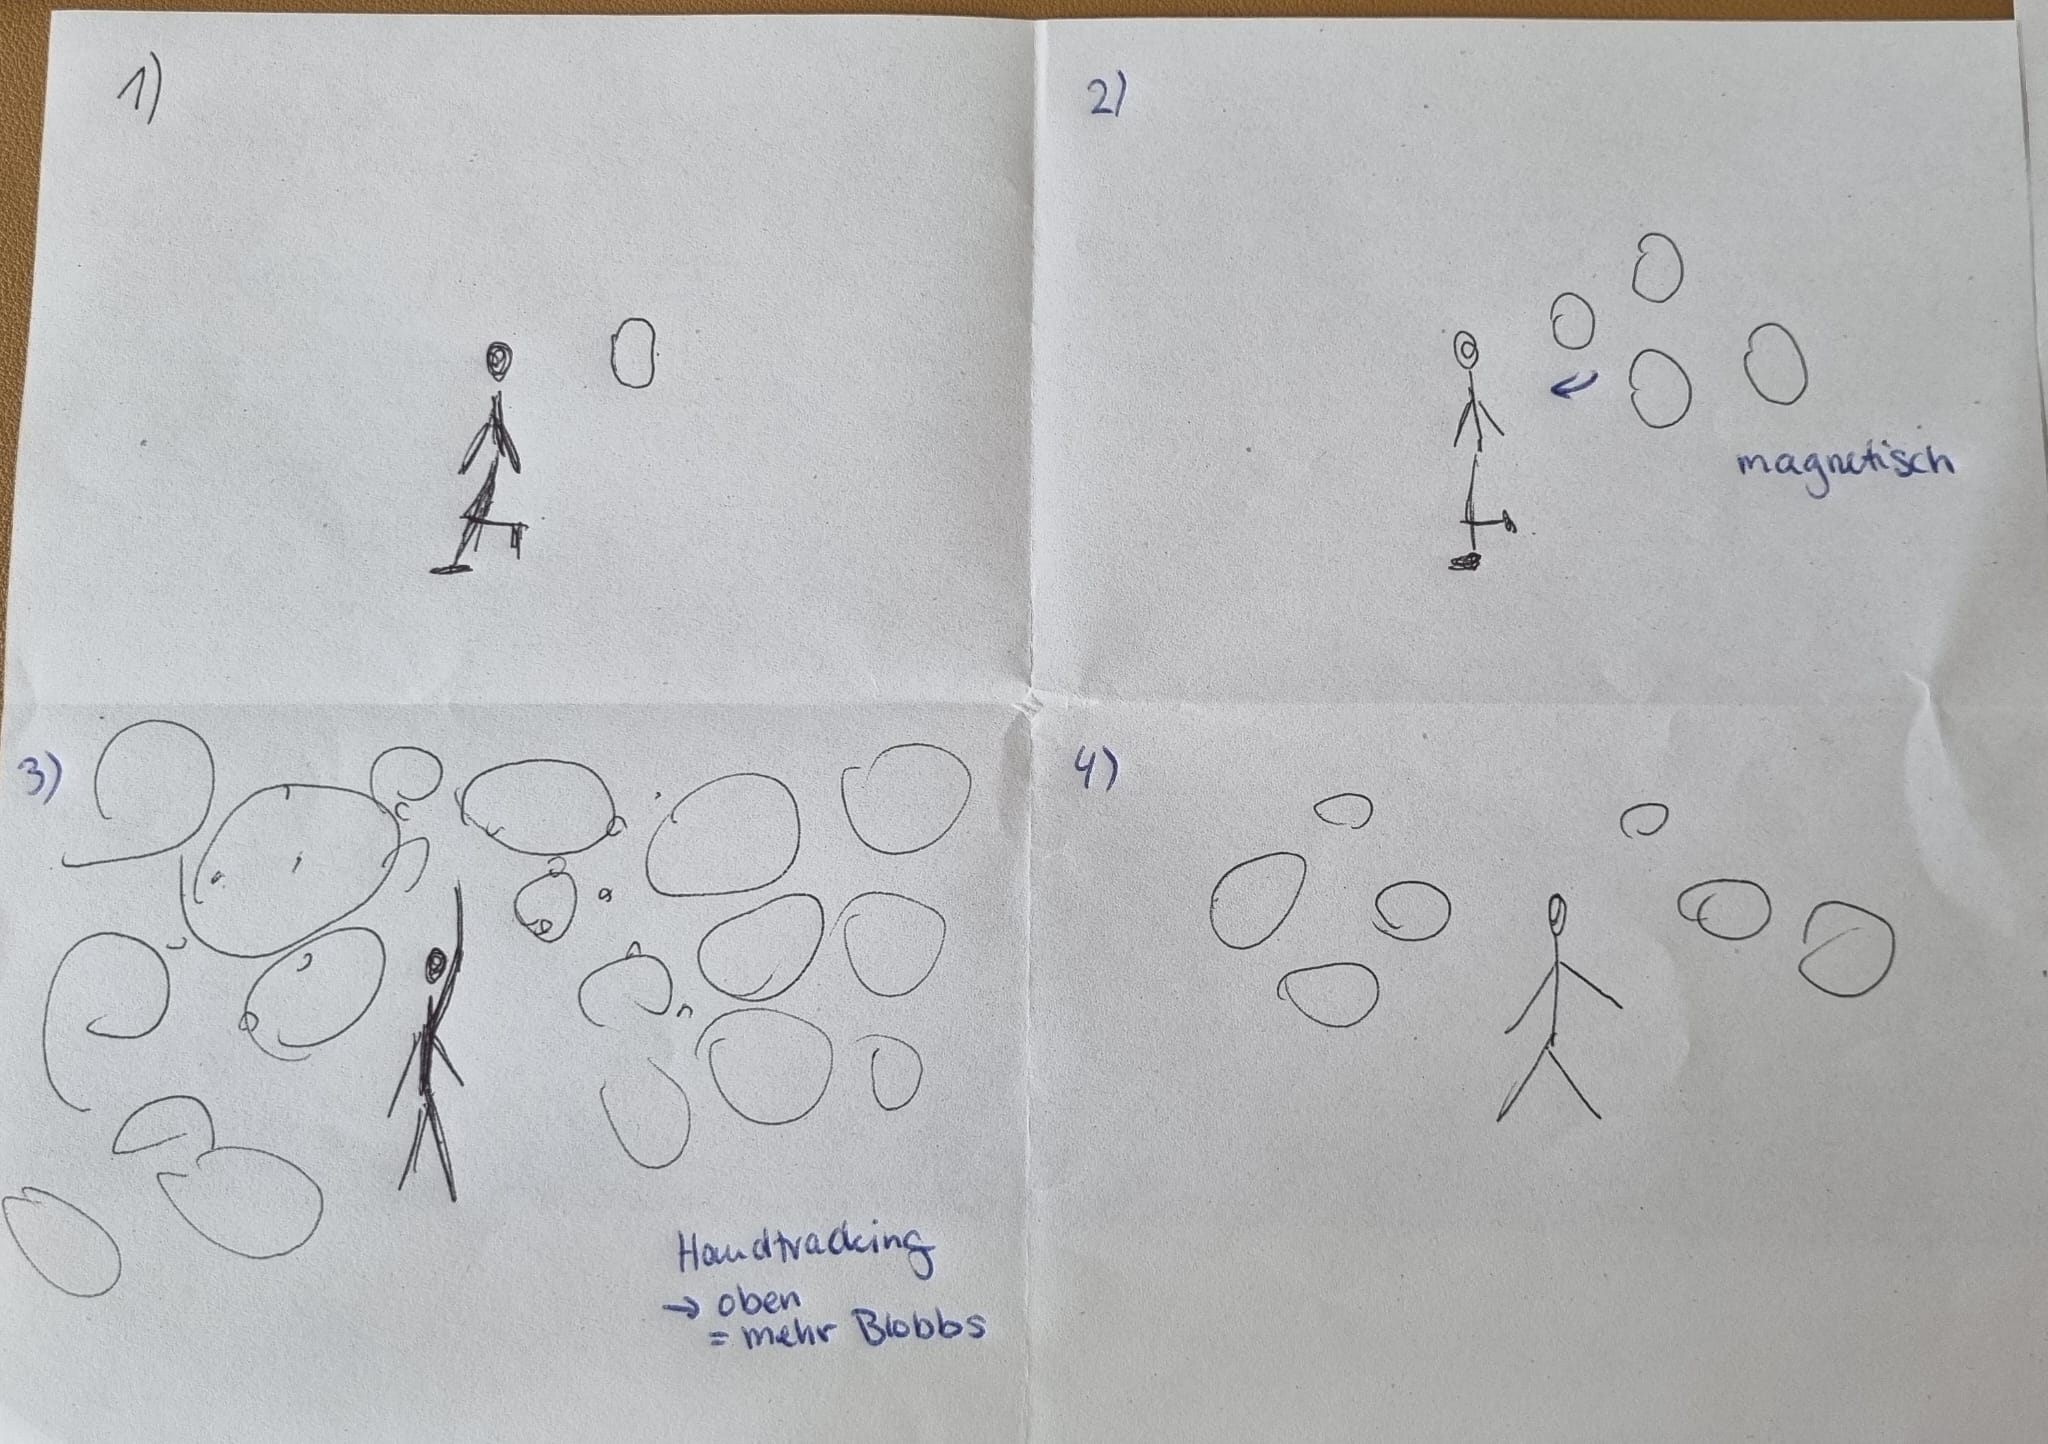
\includegraphics{images/docupictures/Sprint3_1.jpg}%
    }
    \caption{Erstes künsterlisches Konzept der Blobs: Blobs sind magnetisch anziehend/abstoßend zum Künstler}
    \label{fig:scaling_concept}
\end{figure}

\begin{figure}[htbp]
    \centering
    \adjustbox{max width=0.8\textwidth, max height=0.8\textheight, keepaspectratio}{%
        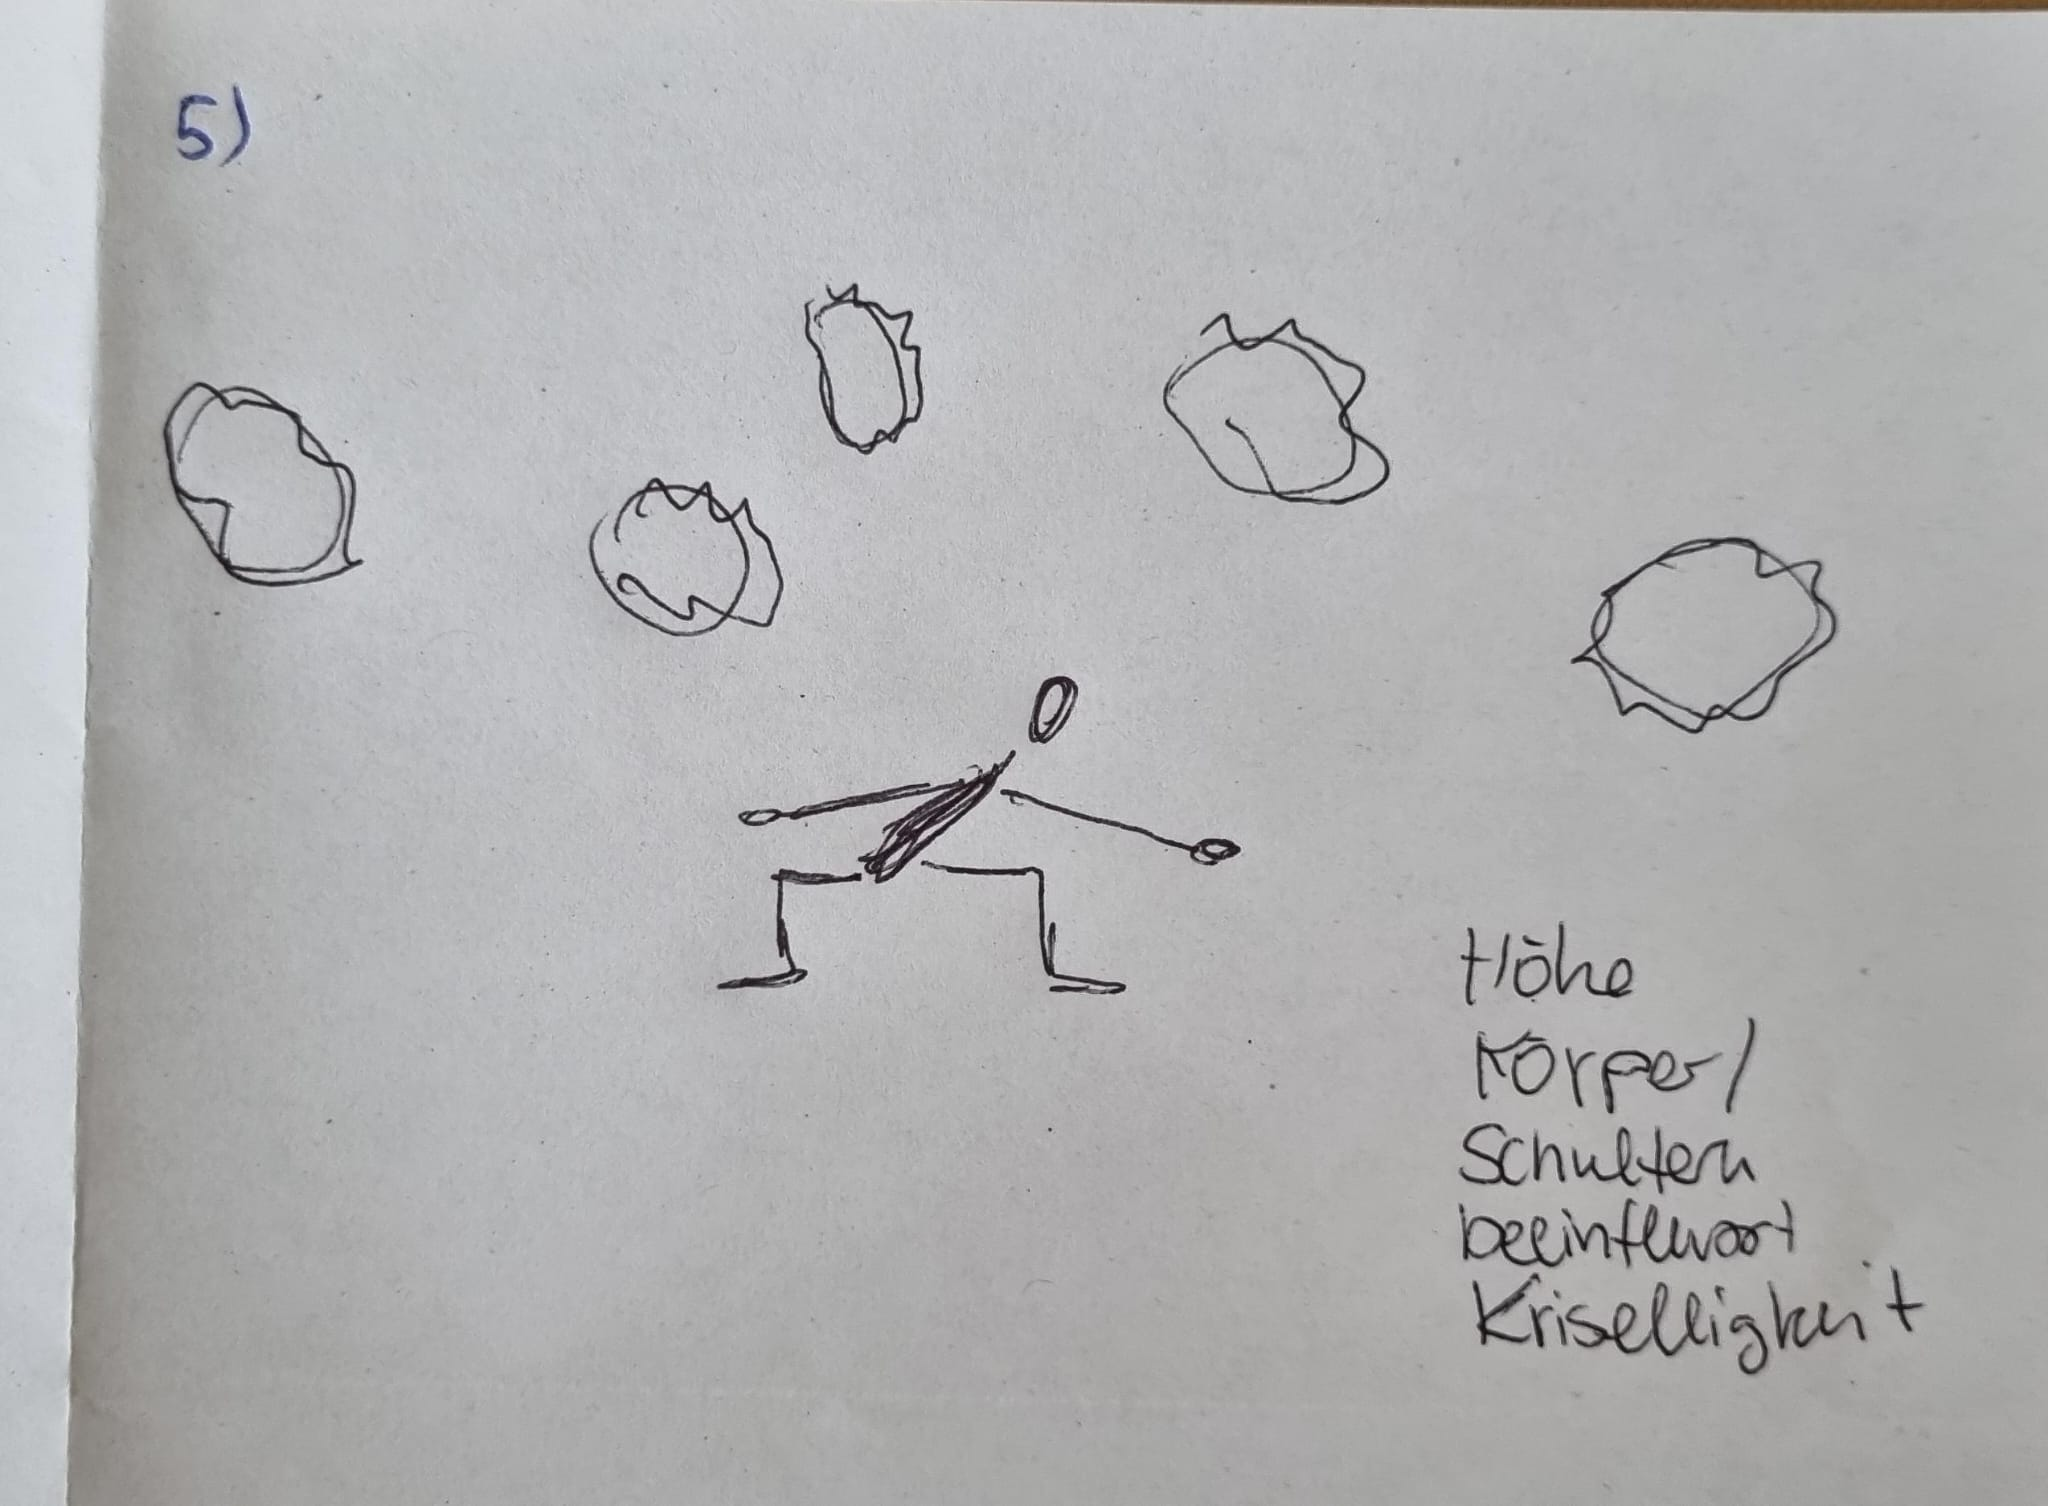
\includegraphics{images/docupictures/Sprint3_2.jpg}%
    }
    \caption{Künsterlisches Konzept, das übernommen wurde: Je nach Position des Performers werden die Blobs krisselig/blitzig oder ruhig dargestellt)}
    \label{fig:external_positioning}
\end{figure}

\begin{figure}[htbp]
    \centering
    \adjustbox{max width=0.8\textwidth, max height=0.8\textheight, keepaspectratio}{%
        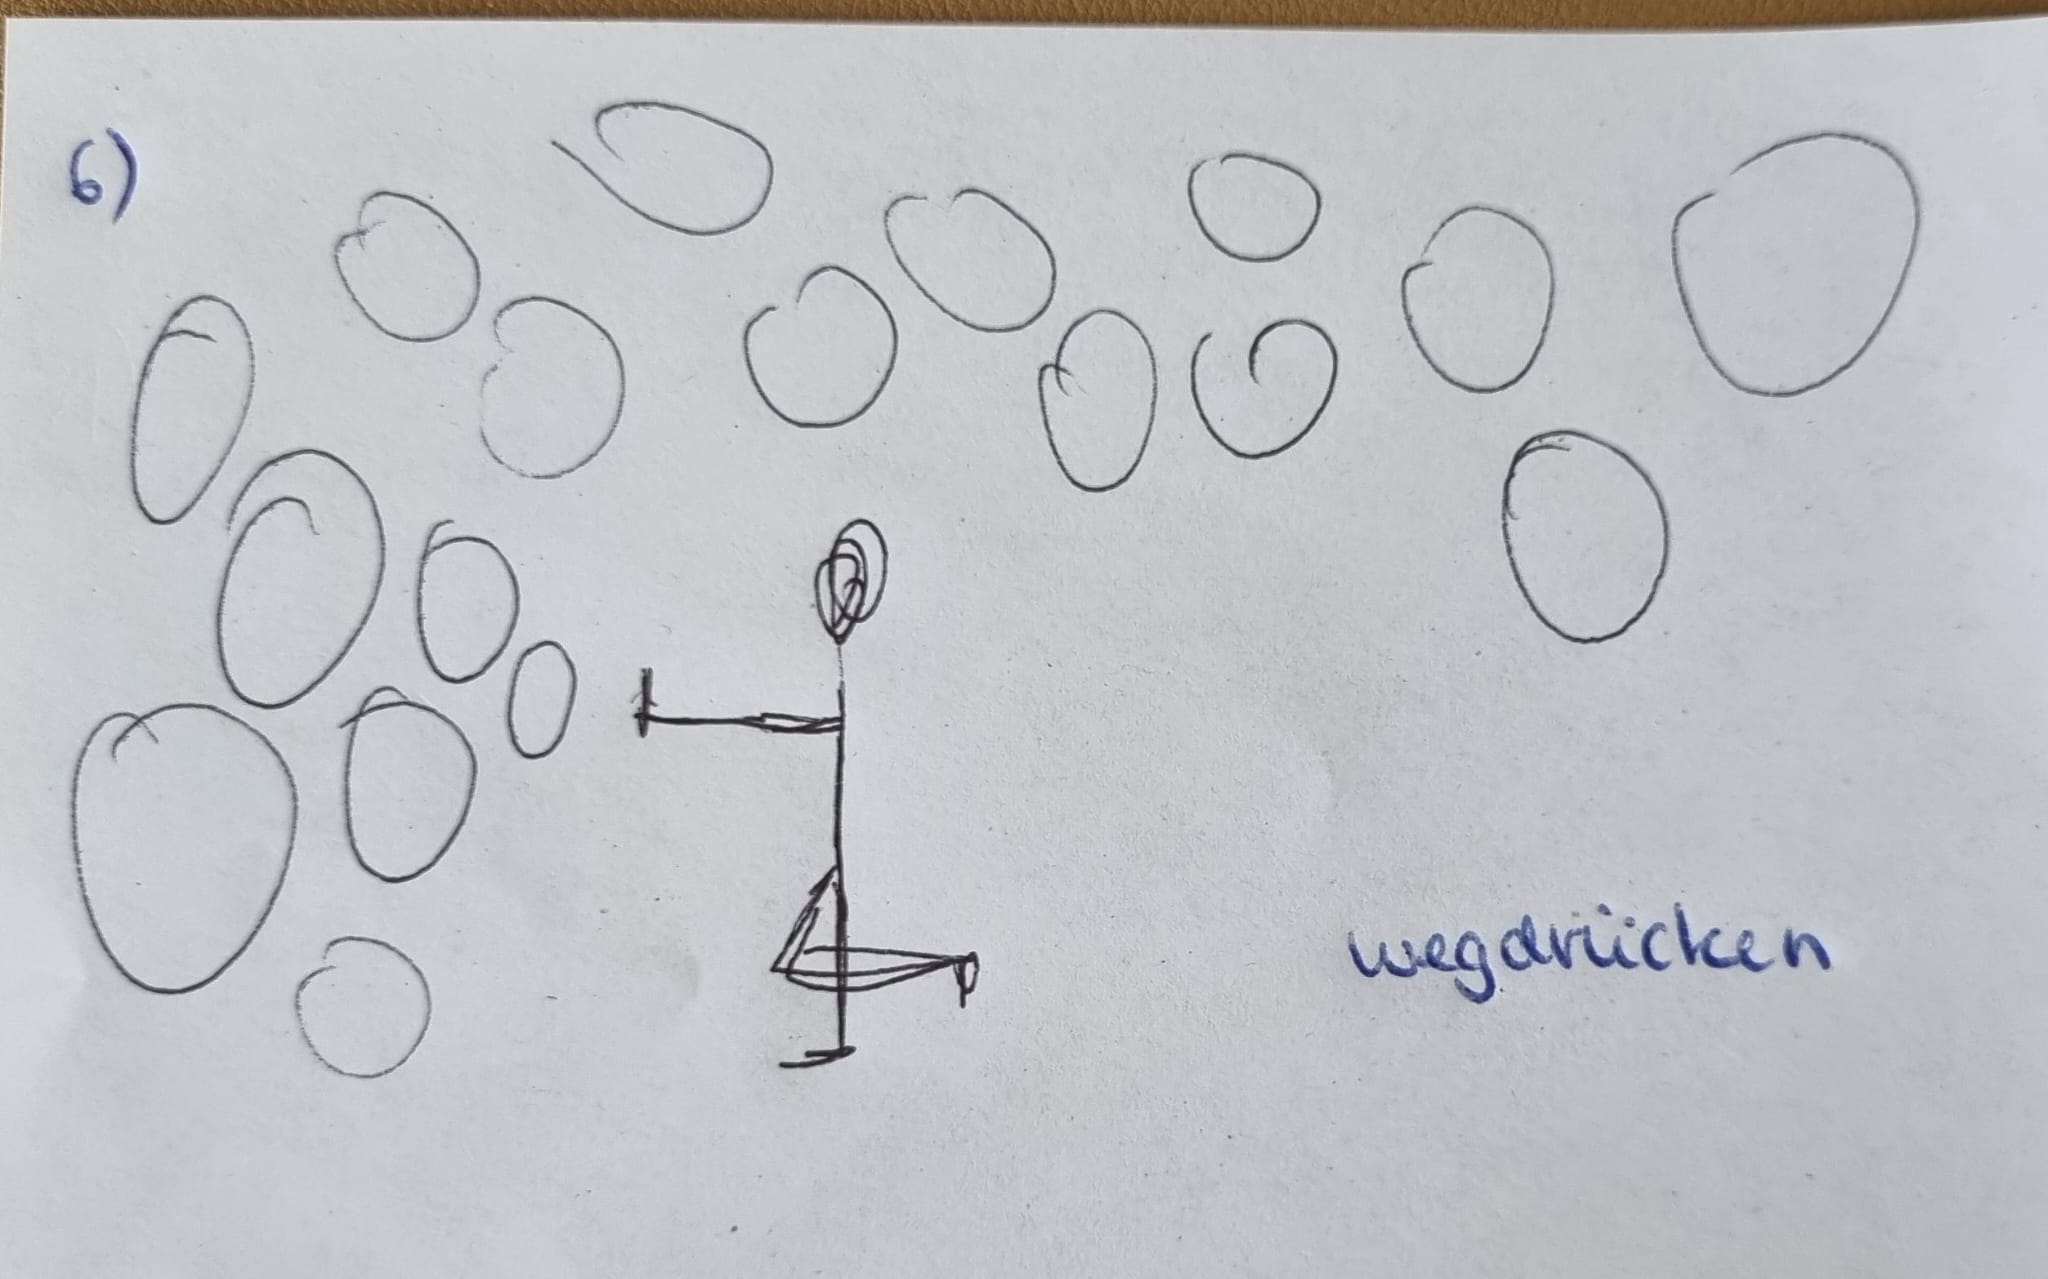
\includegraphics{images/docupictures/Sprint3_3.jpg}%
    }
    \caption{Künsterlisches Konzept, das deprecated wurde, nachdem meine Shader-Solution nicht geklappt hatte: Magnetische Interaktion: Dynamische Visual-Performer-Relation}
    \label{fig:magnetic_interaction}
\end{figure}

\begin{figure}[htbp]
    \centering
    \adjustbox{max width=0.6\textwidth, max height=0.8\textheight, keepaspectratio}{%
        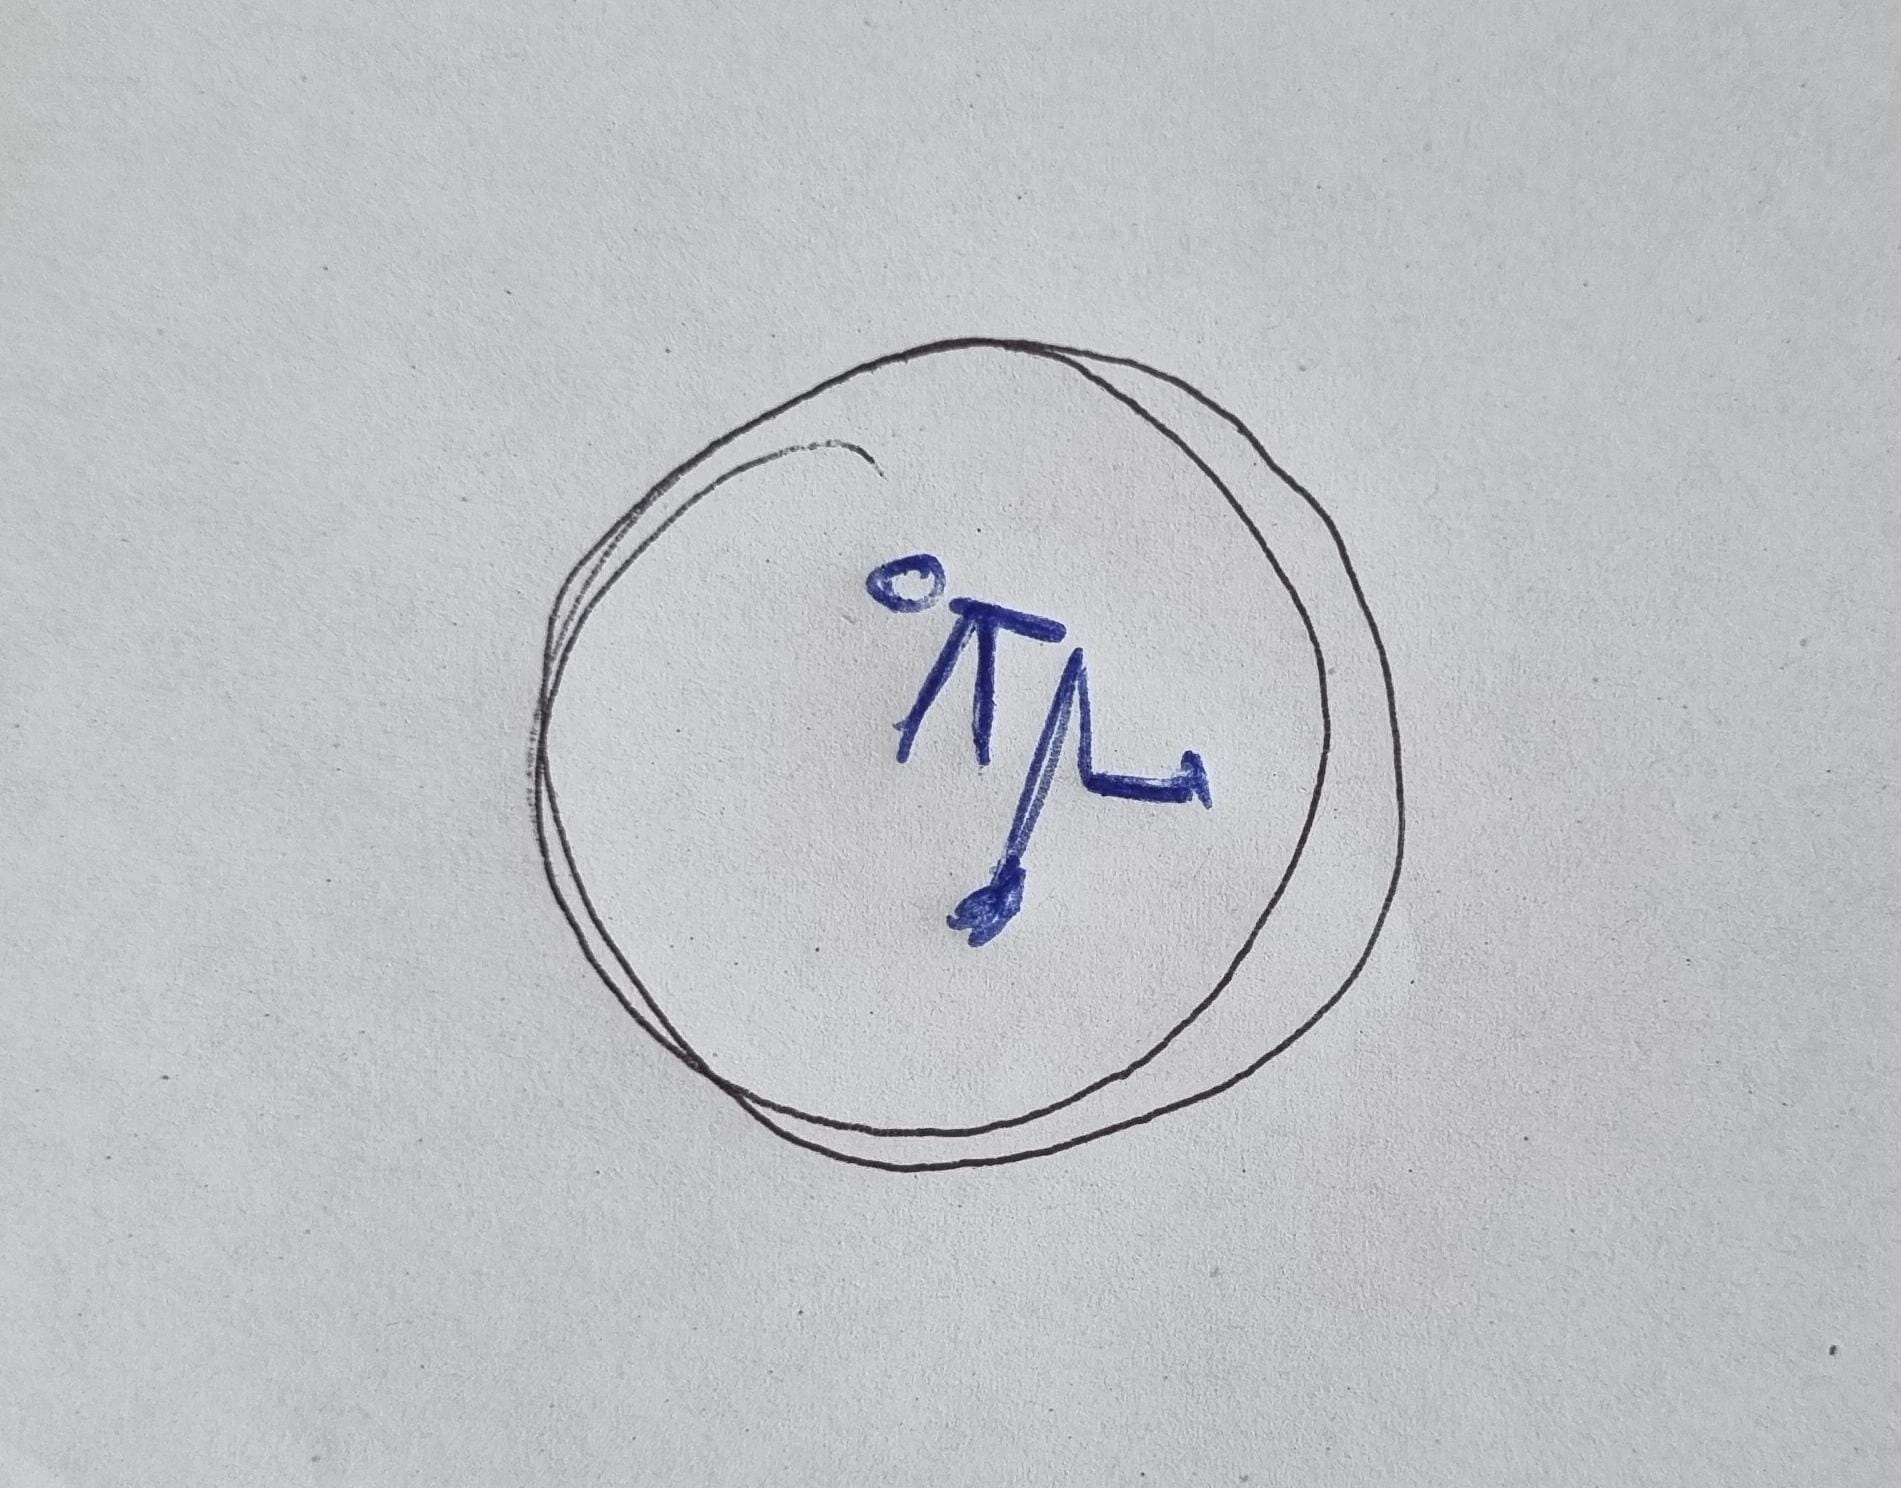
\includegraphics{images/docupictures/Sprint3_4.jpg}%
    }
    \caption{Künsterlisches Konzept, das übernommen wurde: der Performer ist in einem hellen Kreis, und bewegt sich}
    \label{fig:movement_responsive}
\end{figure}

\begin{figure}[htbp]
    \centering
    \adjustbox{max width=0.8\textwidth, max height=0.8\textheight, keepaspectratio}{%
        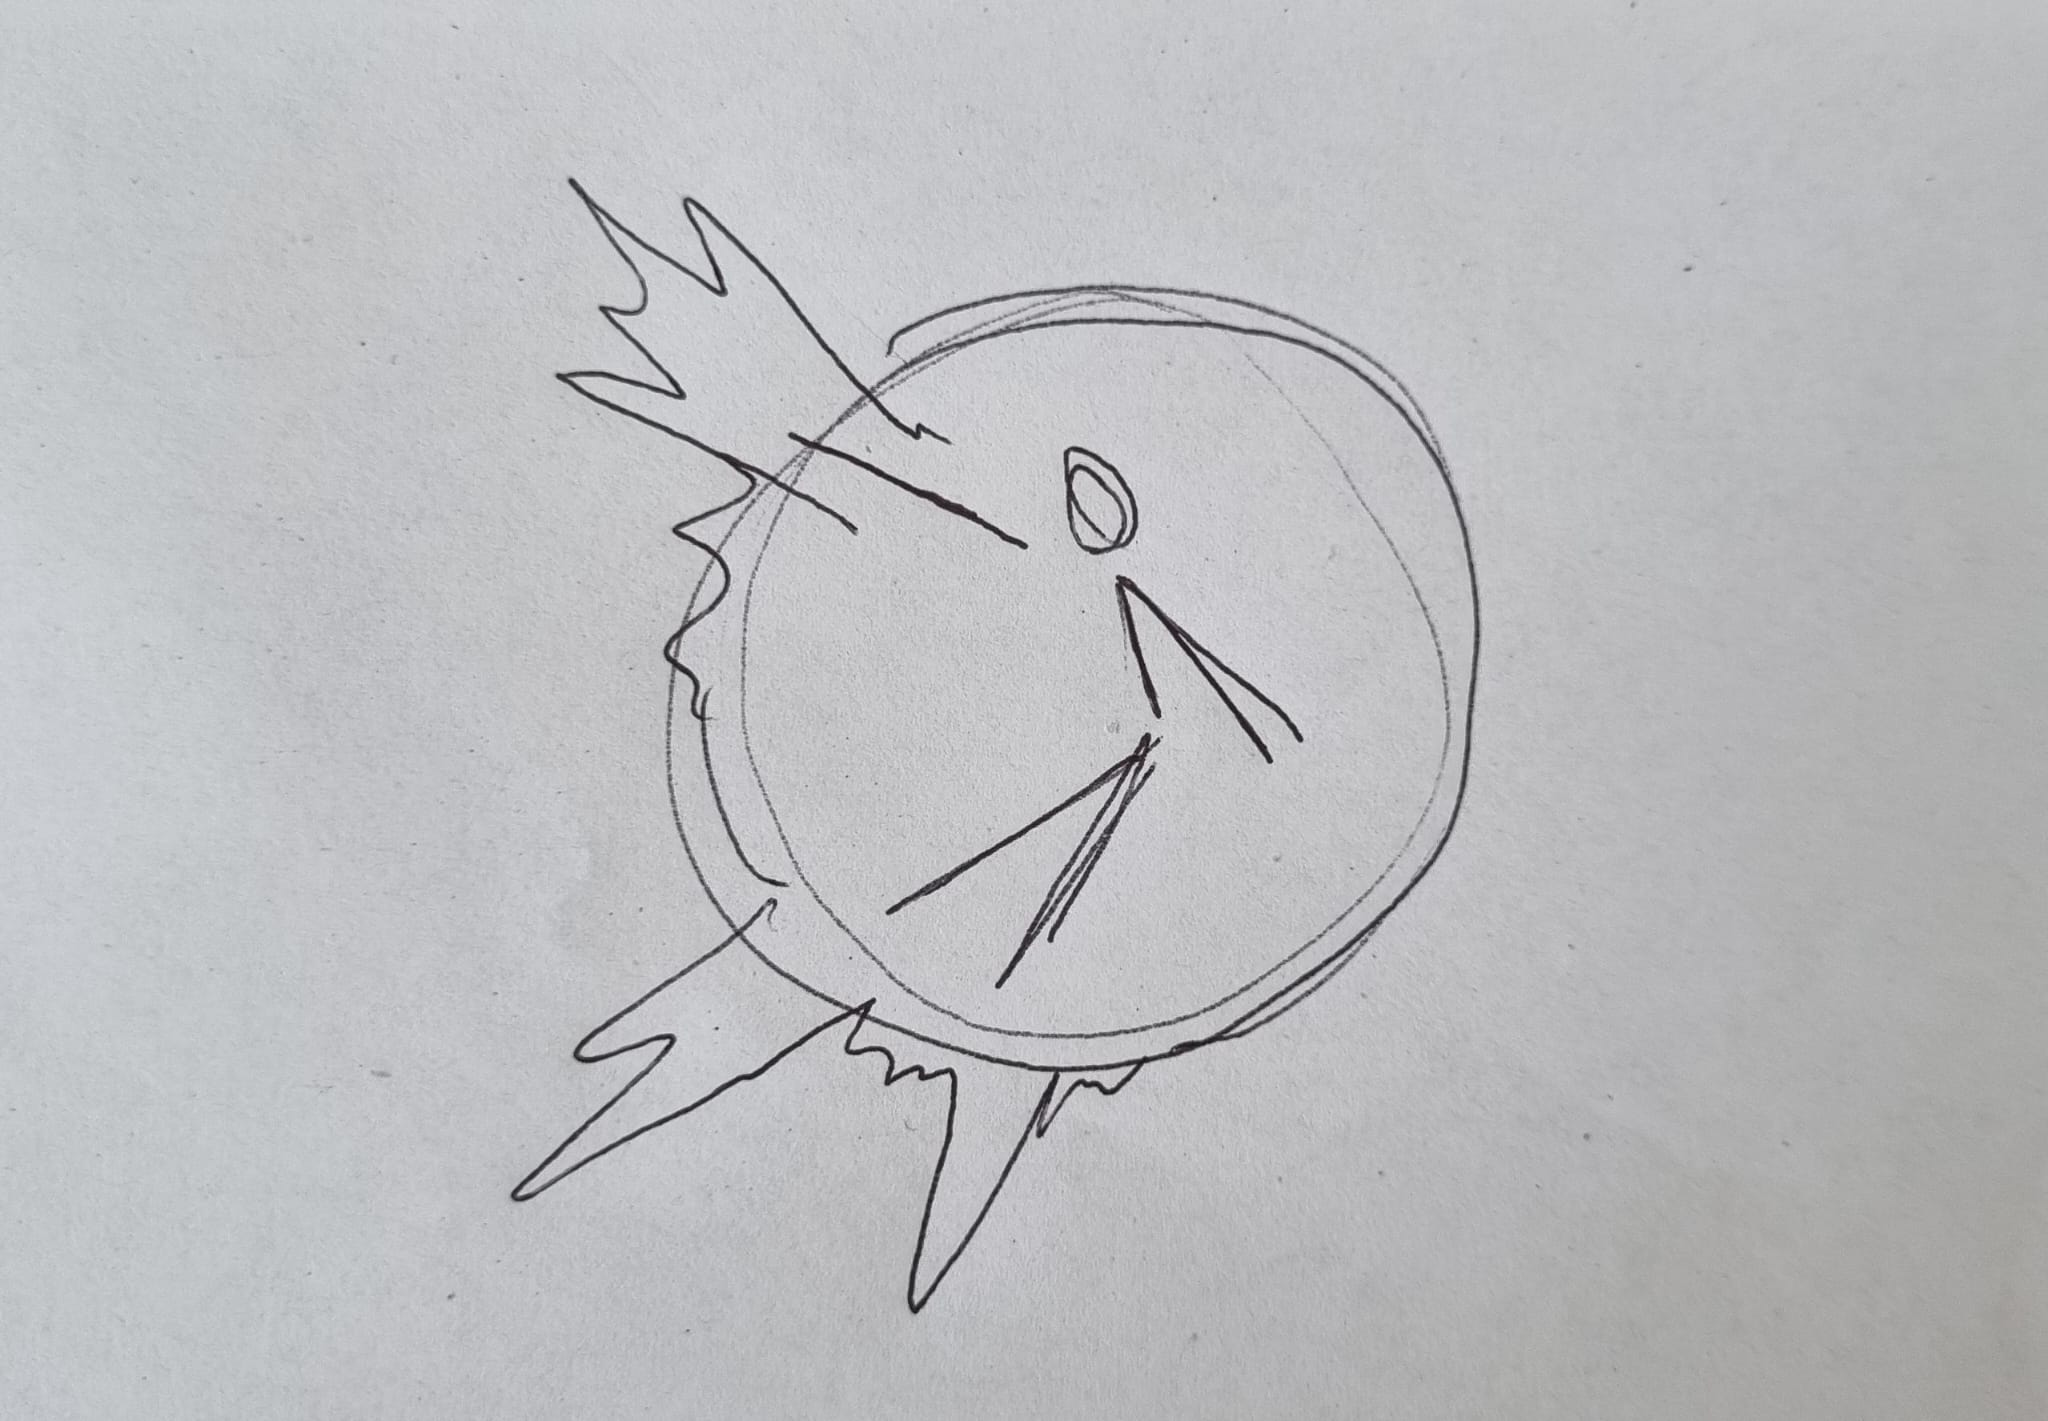
\includegraphics{images/docupictures/Sprint3_5.jpg}%
    }
    \caption{Künsterlisches Konzept, das übernommen wurde: der Performer ist in einem hellen Kreis, und die Visuals brechen interaktiv mit seinen Extremitäten-Koordinaten passend aus}
    \label{fig:composite_effects}
\end{figure}

\textbf{Technische Herausforderungen:}
\raggedright Diese künstlerischen Anforderungen stellten das ursprüngliche System vor erhebliche Performance-Probleme. Die Dual-Source-Architektur erwies sich als zu ressourcenintensiv für komplexe Real-time-Visuals.

\newpage

\subsection{Phase 3: Architektonische Vereinfachung (April 2025)}

\textbf{Strategische Entscheidung:}
\raggedright Angesichts der Performance-Limitationen entschied ich mich für eine radikale Vereinfachung: Vollständige Fokussierung auf MediaPipe als primäres Tracking-System.

\textbf{Systemvereinfachung:}
\begin{itemize}
    \item \textbf{Kinect-Elimination:} Entfernung der nativen Kinect-SDK-Abhängigkeiten
    \item \textbf{MediaPipe-Optimierung:} Direkter RGB-zu-Pose-Pipeline ohne Datenfusion
    \item \textbf{Modulare Architektur:} Plug-and-Play TouchDesigner-Container
    \item \textbf{Performance-Boost:} CPU-Nutzung reduziert
\end{itemize}

\textbf{Unerwartete Erkenntnisse:}
\raggedright Die Vereinfachung führte nicht nur zu besserer Performance, sondern auch zu erhöhter Systemstabilität und einfacherer Wartung – ein klassisches Beispiel für „weniger ist mehr" in der Systemarchitektur.

\subsection{Phase 4: Produktionsvalidierung und Lösungsfindung (Mai 2025)}

\textbf{Beleuchtungsproblem:}
\raggedright Bei den ersten Produktionstests stellte sich heraus, dass intensive Beamer-Projektionen die RGB-Kameras überlasten und MediaPipe funktionsunfähig machen. Ein fundamentales Problem für Live-Performance-Anwendungen.

\textbf{Praxisorientierte Lösung - Infrarot-Pipeline:}
\raggedright Unter Produktionsdruck entwickelte ich eine spezifische Adaptation: Routing des Kinect-Infrarot-Streams (512×424 Pixel, 16-bit) über OBS Virtual Camera direkt zu MediaPipe.


\textbf{Technische Spezifikationen der finalen Lösung:}
\begin{itemize}
    \item \textbf{Input:} Kinect V2 Infrarot-Stream (512×424@30fps)
    \item \textbf{Processing:} OBS Virtual Camera → MediaPipe Pose Detection
    \item \textbf{Output:} TouchDesigner-kompatible Koordinaten-CHOPs
\end{itemize}

\subsection{Phase 5: Spezialisierte Visual-Systeme}

\textbf{Drei finale Implementierungen:}

\raggedright \textit{1. Hand-Feuer-Effekte:}
ParticleGPU-basierte blaue Flammenpartikel, die Handbewegungen in Echtzeit folgen. Implementation extrahiert Hand-Landmarks (MediaPipe Nodes 15/16) und transformiert diese in normalisierte Bildschirmkoordinaten.
Dafür werden per Script die Hand-Node-Positionen in TouchDesigner als Partikel-Emitter genutzt. Die Partikel haben eine Lebenszeit von 1,2 Sekunden und werden basierend auf der Handgeschwindigkeit emittiert.


\textit{2. Adaptive Kopfpartikel:}
Zustandsbasiertes System mit Hand-zu-Schulter-Positionsvergleich. Eine Interpolationsfunktion sorgt für sanfte Übergänge zwischen zwei visuellen Modi.
Die Visuals folgen der Kopf-Node über Setzung des particleGPU offsets von der Mitte des Bildschirms per Script-Mapping.

\textit{3. 64-Spike Radialsystem:}
Hochpräzise Winkelauflösung (5,625°) für Extremitätenerkennung. Polar-Koordinaten-Mapping ermöglicht exakte Richtungstrigger basierend auf Körperhaltung.
Per Skript werden die Hand- und Fußpositionen relativ zum Bildschirmzentrum in Polarkoordinaten umgerechnet. Der atan2-Algorithmus mappt Winkel auf diskrete Spike-Indizes (0-63),
und wird anschließend auf RAMP positionen gemappt, und per connect- disconnect logic anhand der Distanz der Nodes zur Mitte zum Comp verbunden.

\newpage

\subsection{Technische Bilanz}

\textbf{Entwicklungsevolution im Überblick:}
\begin{table}[H]
    \centering
    \adjustbox{width=\textwidth,center}{%
        \begin{tabular}{|l|c|c|c|}
            \hline
            \textbf{Metrik} & \textbf{Initial (Dual-Source)} & \textbf{Vereinfacht (MediaPipe)} & \textbf{Final (IR-Pipeline)} \\ \hline
            CPU-Nutzung & Hoch & Gering & Etwas Mehr als Vereinfacht\\ \hline
            Tracking-Präzision & 75\% & 70\% (RGB) & 90\% (IR) \\ \hline
            Setup-Zeit & 45 Minuten & 15 Minuten & 20 Minuten \\ \hline
            Systemkomplexität & Hoch & Niedrig & Mittel \\ \hline
            Produktionstauglichkeit & Nein & Bedingt & Ja \\ \hline
        \end{tabular}%
    }
    \caption{Systemevolution: Technische Verbesserungen über Entwicklungsphasen (Estimates ohne professionelle Messung!)}
    \label{tab:system_evolution}
\end{table}

\textbf{Lessons Learned:}
\begin{itemize}
    \item \textbf{Constraints fördern Lösungsansätze:} Die Beleuchtungsbeschränkung führte zur infrarot-basierten Adaptation
    \item \textbf{Systemvereinfachung verbessert Robustheit:} MediaPipe-only erwies sich als stabiler als Dual-Source-Ansatz
    \item \textbf{Produktionsvalidierung ist entscheidend:} Reale Umgebungsbedingungen deckten wichtige Designanpassungen auf
    \item \textbf{Interdisziplinarität steigert Qualität:} Zusammenarbeit mit Designerinnen optimierte sowohl technische als auch künstlerische Aspekte
\end{itemize}

Die Entwicklung von M.A.S.K. demonstriert, wie iterative Vereinfachung und praxisorientierte Problemlösung zu eleganten, produktionstauglichen Lösungen führen können. Das finale System ist nicht nur technisch ausgereift, sondern auch konzeptuell klarer und wartungsfreundlicher als die ursprüngliche komplexe Architektur.     % Wie wir es gebaut haben (iterativ)

    \newpage

    \section{Systemarchitektur und Innovation}\label{sec:system}
        % Konsolidierte Darstellung von Systemarchitektur und Produktionsergebnissen

\subsection{Finale Systemarchitektur}

M.A.S.K. implementiert die drei bereits benannten spezialisierte Visualisierungssysteme über eine gemeinsame  (Optional Infrarot-)Tracking-Pipeline. Die modulare Architektur ermöglicht eigenständige Komponenten mit standardisierten Schnittstellen – ein entscheidender Faktor für die erfolgreiche Produktionsintegration.

\subsubsection{Praxisorientierte Lösung: Infrarot-MediaPipe-Pipeline}

\begin{figure}[h]
    \centering
    \includegraphics[width=0.9\textwidth]{images/docupictures/Finished_MediaPipeContainer_mitErklärungen.png}
    \caption{MediaPipe-Container: Vollständige Pipeline-Architektur mit Erklärungen}
    \label{fig:mediapipe_architecture}
\end{figure}

Die zentrale technische Lösung besteht in der Weiterleitung des Kinect V2 Infrarot-Streams über OBS Virtual Camera an MediaPipe. Diese spezifische Adaptation für Produktionsanforderungen reduziert deutlich die Beleuchtungsinterferenzen durch Beamer-Projektionen, die RGB-basierte Systeme beeinträchtigen können.

\textbf{Pipeline-Architektur im Detail:}
\begin{enumerate}
    \item \textbf{Kinect IR-Capture:} 16-bit Tiefendaten werden als Graustufenbild interpretiert
    \item \textbf{OBS-Konversion:} Bit-Shift von 16-bit auf 8-bit für Kompatibilität
    \item \textbf{Virtual Camera Bridge:} Simuliert Webcam-Input für MediaPipe
    \item \textbf{MediaPipe Processing:} Pose-Detection auf IR-Bildern statt RGB
    \item \textbf{TouchDesigner Integration:} Python-Scripts parsen MediaPipe-Output zu CHOP-Daten
\end{enumerate}

\textbf{MediaPipe Debug-Visualisierung (PY\_MediaPipeDebugCirclesForCompTops.py):}
\begin{itemize}
    \item \textbf{Pixel-Koordinaten-Berechnung:} 
    \begin{itemize}
        \item \texttt{x\_px = x\_norm * width - width/2}
        \item \texttt{y\_px = -(y\_norm * height - height/2)} (Y-Achse invertiert)
    \end{itemize}
    \item \textbf{Transform-TOP-Kontrolle:} Dynamische Positionierung von Debug-Kreisen
    \item \textbf{Resolution-Mapping:} Automatische Anpassung an Ausgabe-Auflösung
    \item \textbf{Toggle-Control:} debugValue-CHOP für Ein/Ausblenden der Visualisierung
\end{itemize}

\textbf{Technische Spezifikationen:}
\begin{itemize}
    \item \textbf{Input:} Kinect V2 IR-Stream mit hochauflösender Tiefenauflösung
    \item \textbf{Processing:} Real-time Grayscale-Konversion über OBS Virtual Camera
    \item \textbf{Detection:} MediaPipe Pose-Model optimiert für Infrarot-Input
    \item \textbf{Output:} TouchDesigner-kompatible CHOP-Koordinaten für drei Visual-Systeme
    \item \textbf{Latenz:} Niedrige End-to-End-Latenz unter Produktionsbedingungen
\end{itemize}

\subsection{MediaPipe-Container: Detaillierte technische Implementierung}

\textbf{Interne Container-Architektur:}

Der MediaPipe-Container fungiert als zentrale Tracking-Konversionseinheit zwischen dem MediaPipe-Pose-Detection-System und TouchDesigners nativen CHOP-Datenstrukturen. Die interne Architektur folgt einem modularen Design mit klar definierten Verarbeitungsschichten.

\textbf{Container-Komponenten im Detail:}
\begin{itemize}
    \item \textbf{MediaPipe Interface Layer:} Direkter Zugriff auf MediaPipe-Pose-Detection-API
    \item \textbf{Data Normalization Unit:} Konvertierung von MediaPipe-Landmarks zu normalisierten Koordinaten [0,1]
    \item \textbf{Coordinate System Adapter:} Transformation zwischen verschiedenen Koordinatensystemen (Camera, Screen, World)
    \item \textbf{CHOP Output Generator:} Erzeugung TouchDesigner-kompatibler Channel-Operator-Datenstrukturen
\end{itemize}

\textbf{Container-Zustandsmanagement:}
\begin{itemize}
    \item \textbf{Initialization State:} MediaPipe-Model-Loading und Camera-Input-Validation
    \item \textbf{Active Tracking State:} Kontinuierliche Pose-Detection mit Confidence-Monitoring
\end{itemize}

\textbf{Datenverarbeitungs-Pipeline im Detail:}

Die interne Datenverarbeitung erfolgt in einem mehrstufigen Pipeline-System mit präzise definierten Transformationsschritten:

\textbf{Stufe 1: MediaPipe Raw Data Extraction}
\begin{enumerate}
    \item \texttt{camera\_input ← OBS\_Virtual\_Camera.getFrame()}
    \item \texttt{pose\_results ← MediaPipe.process(camera\_input)}
    \item \texttt{landmarks ← pose\_results.pose\_landmarks}
\end{enumerate}

\textbf{Stufe 2: Coordinate Normalization \& Validation}
\begin{itemize}
    \item \textbf{Landmark-Extraktion:} 33 MediaPipe-Körperpunkte mit x,y,z,visibility-Werten, mit zusäzlicher SpineBase-Approximation
    \item \textbf{Confidence-Filtering:} Schwellenwert-basierte Validierung (Standard: visibility > 0.5 per MediaPipe Container Parameter)
    \item \textbf{Optionale Koordinaten-Normalisierung (wird auch per Python Skript außerhalb gemacht:} Umwandlung zu [0,1]-Bereich für TouchDesigner-Kompatibilität
\end{itemize}

\textbf{Stufe 3: TouchDesigner CHOP Integration}
\begin{itemize}
    \item \textbf{Channel-Mapping:} Jeder Landmark wird zu spezifischen CHOP-Kanälen (x, y, z, confidence)
    \item \textbf{Real-time Update:} Frame-synchrone Aktualisierung aller CHOP-Outputs
    \item \textbf{Data Smoothing:} Optional: Kalman-Filter-Integration für Motion-Smoothing
\end{itemize}

\textbf{Schnittstellen-Dokumentation:}

\textbf{Input-Interfaces:}
\begin{itemize}
    \item \textbf{Camera Input:} OBS Virtual Camera (Grayscale, Echtzeit)
    \item \textbf{Configuration Parameters:} 
    \begin{itemize}
        \item \texttt{model\_complexity}: MediaPipe-Model-Precision (0=Light, 1=Full, 2=Heavy)
        \item \texttt{min\_detection\_confidence}: Minimum-Confidence für Pose-Detection (Standard: 0.5)
        \item \texttt{min\_tracking\_confidence}: Minimum-Confidence für Pose-Tracking (Standard: 0.5)
    \end{itemize}
\end{itemize}

\textbf{Output-Interfaces:}
\begin{itemize}
    \item \textbf{Primary CHOP Outputs:} 33 Landmark-Channels × 4 Dimensionen (x,y,z,visibility)
    \item \textbf{Derived CHOP Outputs:} Spine Base
    \item \textbf{Debug Outputs:} Debug-Visualization-TOPs für Development und Troubleshooting, Head, Extremitäten werden als OUTs aus dem Modul geliefert
\end{itemize}

\textbf{Implementierungsdetails:}

\textbf{Python-Script-Integration:}

Innerhalb des Containers wird ein Skript genutzt, um auffällige grüne Kreise auf das TOP der Visuals genutzt, um die MediaPipe-Landmarks in Echtzeit zu visualisieren. Dieses Skript ist entscheidend für die Debugging-Phase und ermöglicht eine schnelle Validierung der Tracking-Daten.

\item \textbf{PY\_MediaPipeDebugCirclesForCompTops.py:}
\begin{itemize}
    \item Funktion: Real-time Debug-Visualization der MediaPipe-Landmarks
    \item Implementation: Transform-TOP-Kontrolle mit dynamischer Circle-Positionierung
    \item Performance: CPU-optimiert für Echtzeit-Verarbeitung
\end{itemize}

\textbf{Fehlerbehebungs-Leitfaden:}

\textbf{Häufige Container-Probleme und Lösungsansätze:}

\begin{itemize}
    \item \textbf{Problem: MediaPipe-Detection-Failure}
    \begin{itemize}
        \item \textbf{Symptom:} Alle CHOP-Outputs zeigen -1 oder 0-Werte
        \item \textbf{Diagnose:} Confidence-Werte überprüfen, Camera-Input validieren
        \item \textbf{Lösung:} Beleuchtung optimieren, Person vollständig im Frame positionieren
    \end{itemize}
    
    \item \textbf{Problem: Coordinate-System-Mismatch}
    \begin{itemize}
        \item \textbf{Symptom:} Visual-Effects erscheinen an falschen Positionen
        \item \textbf{Diagnose:} Resolution-Mapping in Koordinaten-Transform-Scripts überprüfen
        \item \textbf{Lösung:} \texttt{constant1}-TOP Auflösungswerte mit Ausgabe-Display abgleichen
    \end{itemize}
    
    \item \textbf{Problem: Performance-Degradation}
    \begin{itemize}
        \item \textbf{Symptom:} Frame-Rate < 30fps, erhöhte Latenz
        \item \textbf{Lösung:} MediaPipe-Model-Complexity reduzieren, CHOP-Update-Rate optimieren
    \end{itemize}
\end{itemize}

\textbf{Debug-Workflow:}
\begin{enumerate}
    \item \textbf{MediaPipe-Output-Validation:} Debug-Circles aktivieren über \texttt{debugValue}-CHOP
    \item \textbf{CHOP-Data-Inspection:} Channel-Werte in TouchDesigner-Info-CHOP monitoren
    \item \textbf{Coordinate-Transform-Verification:} Transform-TOP-Outputs visuell validieren
\end{enumerate}

\newpage

\subsection{Drei produktionsvalidierte Visual-Systeme}

\textbf{Gemeinsame Analyse-Pipeline für Trigger-Logik:}

Alle Visual-Systeme nutzen geometrische Beziehungsanalysen zwischen Skelett-Knoten für ihre Trigger-Logik:

\textbf{PY\_NodeDatsToDistanceAngles.py:}
\begin{itemize}
    \item \textbf{Funktion:} Berechnung geometrischer Beziehungen zwischen Skelett-Knoten
    \item \textbf{Features:}
    \begin{itemize}
        \item Extrahiert alle 33 MediaPipe-Landmarks (nose bis right\_heel)
        \item Berechnet SpineBase als Mittelwert der Hüften
        \item Distanzberechnung zwischen definierten Gelenkpaaren
        \item Winkelberechnung über Dot-Product mit Clamping [-1,1]
    \end{itemize}
    \item \textbf{Berechnete Metriken:}
    \begin{itemize}
        \item 13 Distanzen (Schulter-, Ellbogen-, Handgelenk-, Knie-, Knöchel-Abstände)
        \item 14 Winkel (Gelenk-Winkel für Arme, Beine, Hüfte-Hand-Beziehungen)
    \end{itemize}
    \item \textbf{Output:} Direkte Zuweisung zu Constant-CHOPs über \texttt{assignToNode()}
    \item \textbf{Usage:} Trigger-Bedingungen für Visual-Aktivierung und Modus-Wechsel
\end{itemize}

\subsubsection{Visual-System 1: Hand-Feuer-Effekte}

\begin{figure}[h]
    \centering
    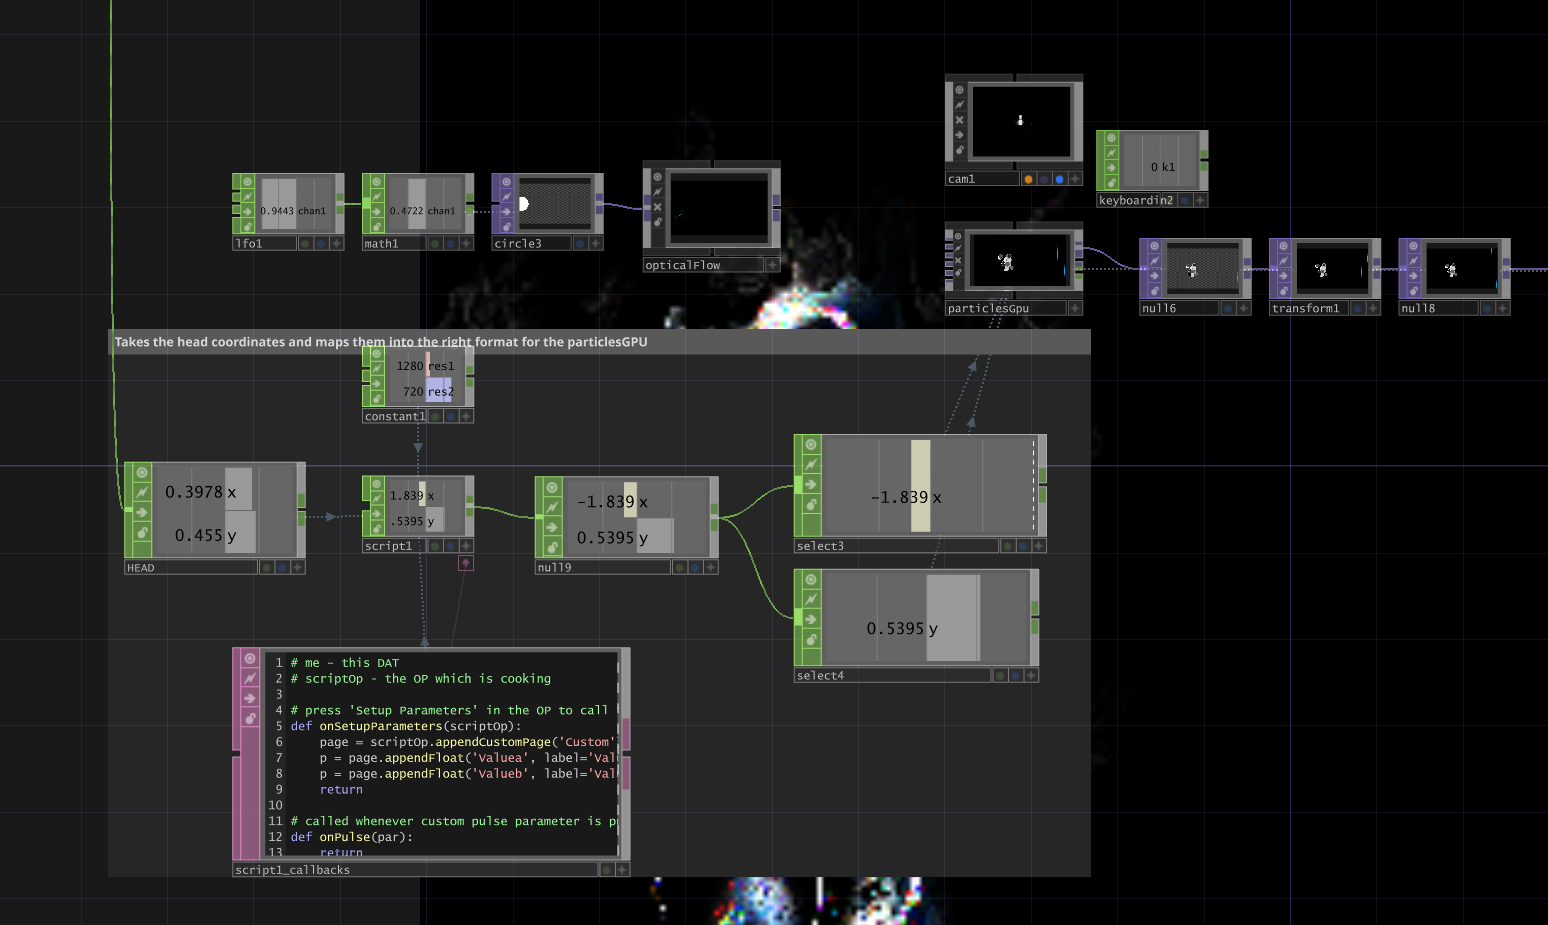
\includegraphics[width=0.8\textwidth]{images/docupictures/NoisyBlob_HEAD_to_ParticleGPU_Translate.png}
    \caption{Hand-Feuer-Implementation: ParticleGPU-basierte Echtzeit-Responsivität}
    \label{fig:hand_fire_system}
\end{figure}

\textbf{Implementation:} TouchDesigners ParticleGPU für blaue Flammenpartikel, extrahiert Hand-Landmarks (MediaPipe Nodes 15/16) und transformiert diese in normalisierte Bildschirmkoordinaten.

\textbf{Koordinaten-Transformation im Detail (PY\_NodeToParticleGPUtranslate.py):}
\begin{itemize}
    \item \textbf{Input:} MediaPipe normalisierte Koordinaten [0,1] vom HEAD-Operator
    \item \textbf{Remapping-Formel:} 
    \begin{itemize}
        \item X: \texttt{tdu.remap(x\_norm, 0.0, 1.0, -9.0, 9.0)}
        \item Y: \texttt{tdu.remap(y\_norm, 0.0, 1.0, 6.0, -6.0)} (invertiert für TouchDesigner)
    \end{itemize}
    \item \textbf{Koordinatenraum:} [-9, 9] horizontal, [-6, 6] vertikal für ParticleGPU-Weltkoordinaten
    \item \textbf{Resolution-Referenz:} constant1-TOP liefert Ausgabeauflösung (1920x1080)
    \item \textbf{Output:} CHOP-Kanäle 'x' und 'y' für direkte ParticleGPU-Force-Steuerung
\end{itemize}

\textbf{Produktionsergebnis:} Robuste Performance nach initialem Setup, fehlerfrei während gesamter Aufnahmezeit.

\subsubsection{Visual-System 2: Adaptive Kopfpartikel}

\textbf{Zustandsmaschine:} Hand-zu-Schulter-Positionsvergleich triggert Partikel-Modus-Wechsel mit Interpolationsfunktion für sanfte Übergänge.

\textbf{Koordinaten-Transformation für Visualisierungs-Modi (PY\_NodeXYzuCentralisedSOPTranslate.py):}
\begin{itemize}
    \item \textbf{Funktion:} Koordinaten-Transformation von normalized zu projection space für rechte Hand
    \item \textbf{Algorithm:} \texttt{x = x\_norm * width/height - 1; y = 0.5 - y\_norm}
    \item \textbf{Input:} \texttt{rechteHand} CHOP mit normalisierten Koordinaten
    \item \textbf{Usage:} SOP-Koordinaten-Mapping für 3D-Geometrie-Positionierung beim Wechsel zwischen Visualisierungs-Modi
    \item \textbf{Integration:} Ermöglicht präzise Partikel-Positionierung relativ zum Performer
\end{itemize}

\textbf{Technische Umsetzung der Zustandslogik (PY\_RelativeNodeValuesToBlended0and1Switch.py):}
\begin{itemize}
    \item \textbf{Vergleichsalgorithmus:} \texttt{logic = 1 if (ly < sy or ry < sy) else 0}
    \begin{itemize}
        \item sy: SpineBase Y-Koordinate (Referenzpunkt)
        \item ly/ry: Linke/Rechte Hand Y-Koordinate
    \end{itemize}
    \item \textbf{Animationssteuerung:} Zeitbasierte Interpolation mit absTime.seconds
    \item \textbf{Blend-Duration:} Dynamisch über blend\_param CHOP (Standard: 0.3s)
    \item \textbf{Interpolationsformel:} \texttt{anim\_value = start + (target - start) * t}
    \item \textbf{Switch-TOP Integration:} Direktes Schreiben auf switch1.par.index
\end{itemize}

\textbf{Produktionserfahrung:} Funktional, aber frontale Kamera-Beamer-Konstellation erfordert häufige Nachkalibrierung – arbeitsintensiv in Produktionsumgebung.

\subsubsection{Visual-System 3: 64-Spike Radialsystem}

\begin{figure}[h]
    \centering
    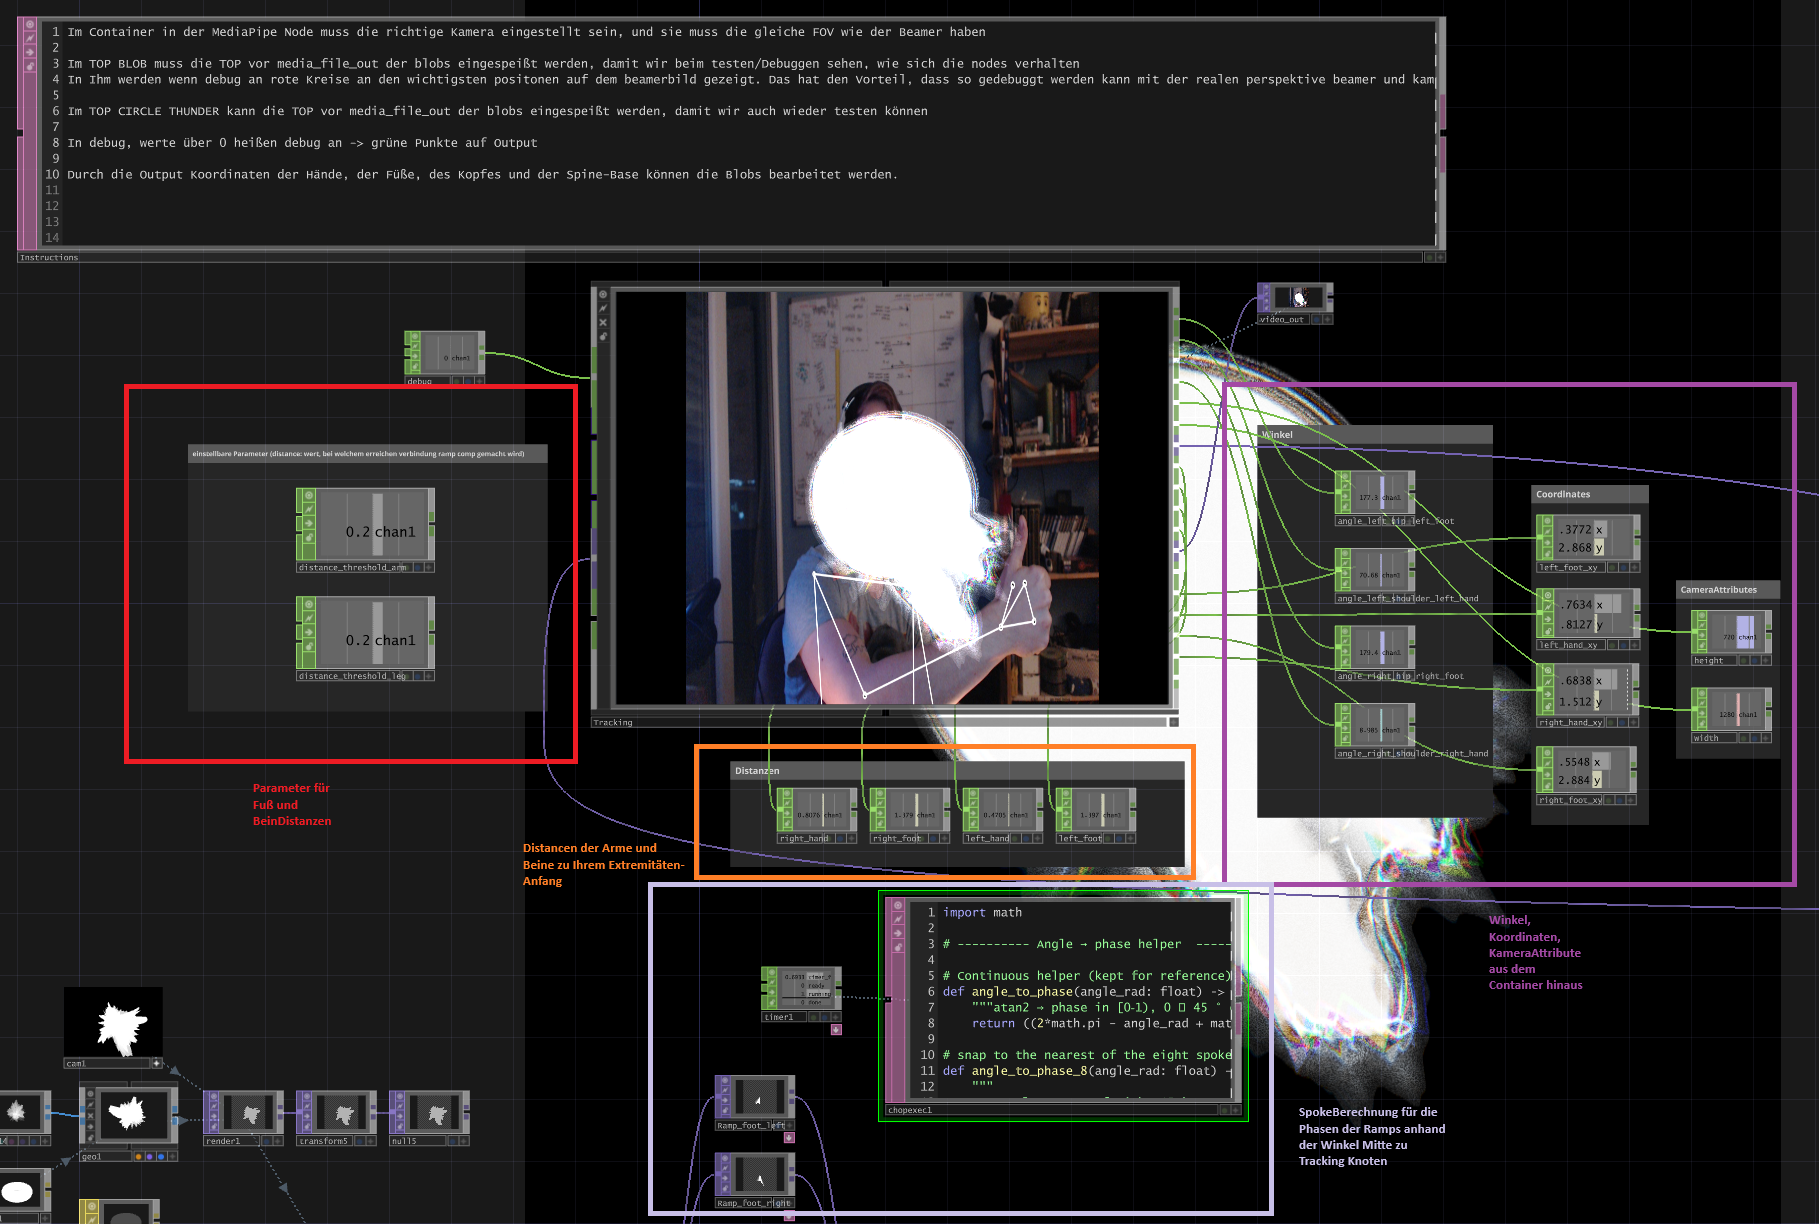
\includegraphics[width=0.8\textwidth]{images/docupictures/TopDown_KreisZuRampsParametisierteBerechnungen.png}
    \caption{64-Spike-System: Polar-Koordinaten-Mapping mit 5,625° Auflösung}
    \label{fig:spike_system_production}
\end{figure}

\textbf{Algorithmus:} atan2-basierte Polar-Koordinaten-Berechnung mappt Hand-/Fußpositionen auf diskrete Spike-Indizes (0-63) mit Intensitäts-Distanz-Korrelation.

\textbf{Detaillierte Polar-Koordinaten-Transformation (PY\_AngleToPhaseSkript):}
\begin{itemize}
    \item \textbf{Aspect-Ratio-Korrektur:} \texttt{x\_wide = x\_raw * aspect} für kreisförmige Distanzen
    \item \textbf{Zentrierung:} \texttt{dx = x\_wide - cx\_wide}, \texttt{dy = y - cy} (cx\_wide = 0.5 * aspect)
    \item \textbf{Polar-Konversion:} 
    \begin{itemize}
        \item \texttt{dist = math.hypot(dx, dy)}
        \item \texttt{angle = math.atan2(dy, dx)}
    \end{itemize}
    \item \textbf{Phase-Mapping (20-Spoke):} \texttt{angle\_to\_phase\_20(angle)}
    \begin{itemize}
        \item Basis: \texttt{((2*$\pi$ - angle + $\pi$/4) / (2*$\pi$)) \% 1.0}
        \item Diskretisierung: \texttt{idx = int(p * 20 + 0.5) \% 20}
        \item 18°-Schritte mit 0/20 = 45° (SE)
    \end{itemize}
    \item \textbf{Schwellenwert-Logik:} Dynamische Verbindung bei \texttt{dist >= threshold}
    \item \textbf{Ramp-TOP-Control:} Automatisches connect/disconnect zu comp15
\end{itemize}

\textbf{Produktionserfolg:} Optimale Performance bei Top-Down-Aufbau, vollständig fehlerfrei während gesamter Aufnahme – das zuverlässigste der drei Systeme.

\subsection{Produktionsvalidierung im Albrecht-Ade-Studio}

\textbf{Zweitägige Intensivtests unter realen Bedingungen:}

\textbf{Tag 1 - System-Integration und Setup-Optimierung:}
\begin{itemize}
    \item \textbf{Infrarot-Modi:} Problemlose Integration, keine Beleuchtungsinterferenzen
    \item \textbf{RGB-Modi:} Funktional unter kontrollierten Lichtbedingungen
    \item \textbf{Setup-Wechsel:} Unter 30 Minuten zwischen Visualisierungsmodi
    \item \textbf{Systemstabilität:} Null kritische Ausfälle während Produktionszeit
\end{itemize}

\textbf{Tag 2 - Vollständige Choreographie-Integration:}
\begin{itemize}
    \item \textbf{1,5 TB Footage:} Vollständige 4K-Aufnahme mit M.A.S.K.-Integration
    \item \textbf{45 Takes:} Kontinuierliche Tracking-Performance ohne Unterbrechungen
    \item \textbf{Professional Workflow:} Nahtlose Integration in Filmproduktions-Pipeline
\end{itemize}

\newpage

\subsection{Quantifizierte Performance-Metriken}

\begin{table}[H]
    \centering
    \begin{tabular}{|l|c|c|c|}
        \hline
        \textbf{System/Modus} & \textbf{Tracking-Genauigkeit} & \textbf{Setup-Aufwand} & \textbf{Produktionsstabilität} \\ \hline
        Top-Down Infrarot & Sehr hoch & Gering & Fehlerlos \\ \hline
        Frontale RGB & Mittel (lichtabhängig) & Hoch & Stabil mit Kalibrierung \\ \hline
        Hand-Feuer-System & Hoch (nach Setup) & Sehr gering & Robust \\ \hline
        64-Spike-System & Sehr hoch (Top-Down) & Minimal & Zuverlässig \\ \hline
        Adaptive Kopfpartikel & Gut (kalibrierungsabhängig) & Mittel & Arbeitsintensiv \\ \hline
    \end{tabular}
    \caption{Produktions-Performance-Vergleich der M.A.S.K.-Systeme}
    \label{tab:production_performance}
\end{table}

\subsection{Technische Lösungsbilanz}

\textbf{Erfolgreiche Lösungsansätze:}

\textbf{Infrarot-Adaptation:} Die spezifisch für Produktionsanforderungen angepasste Infrarot-MediaPipe-Pipeline adressiert effektiv das Problem der Beleuchtungsinterferenz – eine praxisorientierte Lösung mit direkter Produktionsrelevanz.

\textbf{Modulare TouchDesigner-Integration:} Container-basierte Architektur ermöglicht Plug-and-Play-Funktionalität und parallele Entwicklung verschiedener Visualisierungen.

\textbf{Performance-Optimierung:} Signifikante CPU-Nutzungsreduktion durch Systemvereinfachung und Architektur-Refactoring.

\textbf{Produktionserkenntnisse:}

\textbf{Top-Down-Überlegenheit:} Overhead-Tracking erwies sich als robuster und wartungsärmer als frontale Kamera-Setups.

\textbf{Infrarot-Immunität:} Vollständige Beleuchtungsunabhängigkeit ermöglicht kreative Freiheit bei Beamer-Intensität und -Effekten.

\textbf{Setup-Effizienz:} Kurze Setup-Zeiten erfüllen professionelle Produktionsanforderungen.

\subsection{Systemlimitationen und Scope}

\begin{itemize}
    \item \textbf{Single-Person-Tracking:} Bewusste Beschränkung auf einzelne Performer für Choreographie-Fokus.
    \item \textbf{Manuelle Kalibrierung:} Setup-Änderungen erfordern manuellen Kalibrierungsaufwand – akzeptabel für geplante Produktionsabläufe.
    \item \textbf{Hardware-Abhängigkeit:} Kinect V2 als einzige Infrarot-Quelle – robust und kostengünstig ($\approx$90€ gebraucht).
    \item \textbf{Positionierung vs. Konkurrenz:} M.A.S.K. konkurriert nicht mit professionellen Systemen wie OptiTrack, sondern schließt die Lücke zwischen Consumer-Hardware und Profi-Equipment für spezielle Anwendungen unter herausfordernden Beleuchtungsbedingungen.
\end{itemize}

Das M.A.S.K.-System demonstriert erfolgreich, wie constraints-driven engineering zu eleganten, produktionstauglichen Lösungen führt. Die Infrarot-Adaptation entstand aus praktischen Notwendigkeiten und beweist ihre Wirksamkeit durch fehlerfreie Performance unter realen Produktionsbedingungen.  % Finales System

    \tocgroup{Praxisvalidierung}

    \newpage

    \section{Produktionsnachweis}\label{sec:showcase}
        \input{src/Ausführungsdokumentation} % Reale Validierung & Anwendungsfall

    \tocgroup{Erkenntnisse und Lernen}

    \newpage

    \section{Zentrale Erkenntnisse}\label{sec:insights}
        
\subsection{Technische Erkenntnisse}

\textbf{Problemlösung durch Constraints:}

\raggedright Die Infrarot-Pipeline entwickelte sich aus spezifischen Produktionsanforderungen und praktischen Constraints. MediaPipes Verarbeitungsfähigkeit für Infrarot-Daten wurde empirisch validiert und für die Projektanforderungen angepasst. Diese Erfahrung verdeutlichte, wie praxisorientierte Lösungsansätze zur Systemoptimierung beitragen können.

\textbf{Architektonische Evolution:}

\raggedright Der Projektverlauf dokumentiert eine schrittweise Vereinfachung: Von der geplanten Dual-Sensor-Fusion mit Kalman-Filter zu einer reinen MediaPipe-Lösung. Jede Reduktion verbesserte Stabilität und Wartbarkeit. Die finale Architektur ist nicht die technisch komplexeste, aber die praktikabelste.

\textbf{Modularität als Designprinzip:}

\raggedright Die Entscheidung, jeden Aspekt (Tracking, Analyse, Visualisierung) in separate TouchDesigner-Container zu kapseln, erwies sich als fundamental. Sie ermöglichte nicht nur parallele Entwicklung, sondern macht das System zukunftssicher: Neue Tracking-Technologien können ohne Änderung der Visualisierungslogik integriert werden.

\textbf{Projektmanagement im interdisziplinären Kontext:}

\textbf{Adaptive Planung:}

\raggedright Die Sprint-Struktur musste mehrfach angepasst werden. Choreographische Anforderungen entstanden organisch während der Proben, nicht durch Requirements Engineering. Sprint 3 wurde komplett umgeplant, als die handgezeichneten Visual-Konzepte eintrafen. Diese Flexibilität war keine Schwäche, sondern Stärke des Prozesses.

\textbf{Dokumentation als Kommunikationswerkzeug:}

\raggedright Die parallele Dokumentation diente nicht nur der Nachvollziehbarkeit, sondern wurde zum primären Kommunikationsmedium mit den Stakeholdern. Screenshots und Diagramme überbrückten die Sprachbarriere zwischen Technik und Kunst effektiver als verbale Erklärungen.

\textbf{Solo-Development-Strategien:}

\raggedright Als Alleinentwickler musste ich spezifische Strategien für die Stakeholder-Kommunikation entwickeln:

\textbf{Erfolgreiche Ansätze:}
\begin{itemize}
\item \textbf{Regelmäßige Demo-Sessions:} Konkrete Fortschritte reduzierten Stakeholder-Unsicherheit
\item \textbf{Transparente Dokumentation:} GitHub-Repository und .toe-Dateien als Kommunikationsbasis
\item \textbf{Proaktive Problem-Kommunikation:} Frühe Information bei technischen Herausforderungen
\item \textbf{Sprint-synchronisierte Updates:} Strukturierte 2-3 Wochen Kommunikationsrhythmus
\end{itemize}

\textbf{Herausforderungen der Solo-Entwicklung:}
\begin{itemize}
\item \textbf{Isolation bei technischen Problemen:} Eigenständige Problemlösung zeitaufwändig
\item \textbf{Stakeholder-Erwartungsmanagement:} Balance zwischen Ambition und Realisierbarkeit
\item \textbf{Dokumentations-Overhead:} Umfassende Dokumentation für interdisziplinäre Kommunikation
\end{itemize}

\textbf{Kollaboration über Disziplingrenzen:}

\textbf{Visuelle Kommunikation:}

\raggedright Die wichtigste Herausforderung war die Übersetzung zwischen künstlerischer Vision und technischer Implementation. „Es soll aussehen wie Gedanken, die explodieren" musste in Partikel-Emissionsraten und Geschwindigkeitsvektoren übersetzt werden. Die Lösung: Rapid Prototyping mit sofortigem visuellem Feedback.

\textbf{Gegenseitiges Lernen:}

\raggedright Das Filmteam lernte technische Constraints zu respektieren (MediaPipe braucht Kontrast), ich lernte künstlerische Prioritäten zu verstehen (Effekt vor Präzision). Diese gegenseitige Bildung war wertvoll über das Projekt hinaus.

\textbf{Iterative Stakeholder-Integration:}

Schlüsselmomente der Zusammenarbeit prägten die Entwicklungsrichtung:
\begin{itemize}
\item \textbf{Frühe Expertenberatung:} Technical Review (17.01.2025) definierte Projektrichtung
\item \textbf{Stakeholder-Integration:} Choreographie-Meeting (10.03.2025) prägte Entwicklung
\item \textbf{Iterative Validation:} Kontinuierliche Demo-Sessions verhinderten Fehlentwicklung
\item \textbf{Lösungen durch Notwendigkeit:} Produktionsanforderungen führten zu praktischen technischen Anpassungen
\end{itemize}

\textbf{Produktionsumgebung und Systemvalidierung:}

\textbf{Echtzeit-Anforderungen:}

\raggedright Die Produktionsumgebung erforderte robuste Systemarchitektur mit minimalen Ausfallzeiten. Entwickelte Debug-Visualisierungen dienten gleichzeitig als Produktionsmonitoring-Tools. Die Echtzeit-Skelett-Overlays erwiesen sich als essentiell für die operative Systemüberwachung während der Aufnahmen.

\textbf{Professionelle Koordination:}

\raggedright Die Integration in professionelle Produktionsabläufe erforderte strukturierte Kommunikation technischer Anforderungen mit der Produktionsleitung. Diese Koordination zwischen technischen Systemanforderungen und kreativen Produktionszielen war ein wichtiger Aspekt des interdisziplinären Projektmanagements.

\textbf{Professionelle Entwicklung:}

\textbf{Vollständige Projektverantwortung:}

\raggedright Als einziger Entwickler trug ich die komplette technische Verantwortung. Jede Architekturentscheidung, jede Optimierung, jeder Workaround – alles lag in meiner Hand. Diese Erfahrung der vollständigen Ownership war gleichzeitig belastend und ermächtigend.

\textbf{Realistische Selbsteinschätzung:}

\raggedright Das Projekt lehrte mich, eigene Grenzen zu erkennen und zu kommunizieren. M.A.S.K. konkurriert nicht mit industriellen Motion-Capture-Systemen – und das ist in Ordnung. Diese Ehrlichkeit ermöglichte fokussierte Entwicklung statt feature creep.

\textbf{Nachhaltige Learnings:}

Drei Erkenntnisse prägen meine weitere Arbeit:

\textbf{1. Pragmatismus schlägt Perfektionismus:} Die funktionierende 80\%-Lösung ist wertvoller als die theoretische 100\%-Lösung.

\textbf{2. Interdisziplinarität erfordert Demut:} Andere Fachbereiche haben eigene Exzellenzkriterien, die respektiert werden müssen.

\textbf{3. Constraints fördern Kreativität:} \raggedright Die Limitierungen (Budget, Hardware, Zeit) zwangen zu alternativen Lösungen, die in einem ressourcenreichen Umfeld nie entstanden wären.

Die eigenständige Entwicklung von M.A.S.K. demonstriert, wie strukturierte Kommunikation und agile Methoden auch bei Solo-Projekten zu erfolgreicher interdisziplinärer Zusammenarbeit führen können.


    \newpage

    \section{Fazit und Beiträge}\label{sec:conclusions}
        \subsection{Projektergebnis}

M.A.S.K. demonstriert, dass spezialisierte Motion-Capture-Lösungen mit Consumer-Hardware realisierbar sind. Das System adressiert erfolgreich die spezifische Herausforderung des Trackings unter intensiver Bühnenbeleuchtung und macht diese Technologie für Projekte mit begrenztem Budget zugänglich.

\subsection{Technischer Beitrag}

Die Infrarot-MediaPipe-Pipeline stellt eine praxisorientierte Lösung für spezifische Produktionsanforderungen dar. Während professionelle Systeme auf spezialisierte Hardware setzen, nutzt M.A.S.K. die verfügbare Infrarot-Funktionalität der Kinect V2 in Kombination mit MediaPipes Machine-Learning-Modell. Diese Adaptation wurde spezifisch für die Projektanforderungen entwickelt und validiert.

Die modulare TouchDesigner-Architektur ermöglicht es anderen Entwicklern, einzelne Komponenten für eigene Projekte zu adaptieren. Das GitHub-Repository enthält nicht nur Code, sondern auch die komplette Entwicklungshistorie inklusive verworfener Ansätze – wertvoll für Lernende.

\subsection{Praktische Relevanz}

Für Bildungseinrichtungen und unabhängige Künstler bietet M.A.S.K. eine realistische Alternative zu kommerziellen Systemen. Die Hardware-Kosten beschränken sich auf circa 100 Euro für gebrauchte Kinect V2 Hardware, wobei zusätzliche Software-Infrastruktur (TouchDesigner, OBS Studio) und Entwicklungszeit je nach Projektanforderungen zu kalkulieren sind.

Die erfolgreiche Produktion von "Echoes of the Mind" validiert die Praxistauglichkeit. Das System bewältigte 45 Takes über zwei Produktionstage ohne kritische Ausfälle – ein Beweis für die Stabilität der gewählten Architektur.

\subsection{Limitierungen und Kontext}

M.A.S.K. ersetzt keine professionellen Motion-Capture-Systeme. Für Anwendungen, die Millimeterpräzision, Multi-Person-Tracking oder 360-Grad-Erfassung erfordern, bleiben kommerzielle Lösungen überlegen. Diese Einschränkung ist bewusst: Durch Fokussierung auf einen spezifischen Use-Case konnte eine robuste Lösung entstehen.

Technische Grenzen:
\begin{itemize}
    \item Single-Person-\\Tracking only
    \item Frontalerfassung (keine 360-Grad-Abdeckung)
    \item Manuelle Kalibrierung bei Setup-Änderungen
    \item Abhängigkeit von MediaPipes Modell-Limitierungen
\end{itemize}

\subsection{Weiterentwicklungspotenzial}

Die Open-Source-Natur des Projekts lädt zu Erweiterungen ein:

\textbf{Kurzfristig:}
\begin{itemize}
    \item Automatische Kalibrierungsroutinen
    \item Weitere Visual-Effekte für die bestehende Pipeline
    \item Verbessertes Handling von Okklusionen
\end{itemize}

\textbf{Mittelfristig:}
\begin{itemize}
    \item Integration neuerer ML-Modelle (MediaPipe Holistic)
    \item Multi-Sensor-Fusion mit IMUs oder LiDAR
    \item Echtzeit-Performance-Metriken
\end{itemize}

\textbf{Langfristig:}
\begin{itemize}
    \item Portierung auf andere Plattformen (Mac, Linux)
    \item Web-basierte Konfigurationsoberfläche
    \item Integration in Game-Engines
\end{itemize}

\subsection{Breitere Implikationen}

Die zunehmende Verschmelzung von Performance-Kunst und digitaler Technologie erfordert zugängliche Werkzeuge. M.A.S.K. zeigt, dass akademische Projekte diese Lücke füllen können, wenn sie sich auf praktische Probleme fokussieren statt auf theoretische Vollständigkeit.

Die Infrarot-Lösung könnte Anwendungen über die Kunst hinaus finden: Physiotherapie-Überwachung, Sporttechnik-Analyse oder barrierefreie Interfaces könnten von der Beleuchtungsunabhängigkeit profitieren.

\subsection{Abschließende Bewertung}

M.A.S.K. ist eine praxisorientierte Lösung, die bewährte Technologien für spezifische Anwendungsanforderungen kombiniert. Das System entstand aus konkreten Produktionsnotwendigkeiten und demonstriert, wie interdisziplinäre Zusammenarbeit zu funktionsfähigen technischen Lösungen führen kann. Der Wert liegt in der durchdachten Integration verfügbarer Komponenten und der bewiesenen Produktionstauglichkeit.

Das Projekt erfüllte seinen Zweck: Es ermöglichte "Echoes of the Mind" und bleibt als Open-Source-Werkzeug für andere verfügbar. In einer Welt, in der Technologie oft als Selbstzweck entwickelt wird, ist diese zielgerichtete Pragmatik vielleicht die wichtigste Stärke von M.A.S.K.

    \tocgroup{Technische Dokumentation}

    % Anhänge für detaillierte technische Informationen
    \appendix

    \newpage

    \section{Vollständiges Code-Repository}\label{app:code}
        \input{src/anhang_code_übersicht}

    \newpage

    \section{Team und Kommunikation}\label{app:team}
        \subsection{Professionelle Kollaboration zwischen Hochschulen}

\subsubsection{Interdisziplinäres Entwicklungsteam}

\textbf{Technische Führung - Hochschule Reutlingen:}
\begin{itemize}
    \item \textbf{Entwickler:} Marty Lauterbach (Sole Developer, Technische Projektleitung)
    \item \textbf{Rolle:} System-Architektur, MediaPipe-Integration, TouchDesigner-Pipeline-Entwicklung
    \item \textbf{Verantwortung:} Vollständige technische Implementation als einziger Entwickler der Hochschule
    \item \textbf{Entwicklung:} Eigenständige Umsetzung der Infrarot-MediaPipe-Pipeline
\end{itemize}

\textbf{Kreative Partner - Filmakademie Baden-Württemberg:}
\begin{itemize}
    \item \textbf{Designerinnen:} Maja Litzke und Rahel Fundinger (Creative Direction, Künstlerische Leitung)
    \item \textbf{Projektkontext:} "Echoes of the Mind" - Cinematographische Tanzproduktion über mentale Zustände
    \item \textbf{Kollaborationsqualität:} Intensive interdisziplinäre Partnerschaft zwischen Technik und Kunst
    \item \textbf{Kommunikation:} Regelmäßige Sprint-Meetings und kontinuierlicher fachlicher Austausch
\end{itemize}

\textbf{Interdisziplinäre Konstellation:}
Diese Kooperation zwischen einem Hochschulentwickler und erfahrenen Filmakademie-Designerinnen ermöglichte eine produktive Synthese aus technischer Entwicklung und künstlerischer Vision.

\subsubsection{Betreuung und Beratung}

\textbf{Hochschule Reutlingen:}
\begin{itemize}
    \item \textbf{Projektbetreuung:} Anja Hartmann (Akademische Betreuung, Bewertung)
    \item \textbf{Fachberatung:} Niklas Zidarov Digital Art (Technische Beratung, 17.01.2025)
    \item \textbf{Rolle:} Akademische Unterstützung, Qualitätssicherung
\end{itemize}

\textbf{Produktionsumgebung:}
\begin{itemize}
    \item \textbf{Albrecht-Ade-Studio:} Produktionsstudio der Filmakademie
    \item \textbf{Technische Crew:} Kamerateam, Beleuchtung, Tontechnik
    \item \textbf{Equipment-Management:} Hardware-Bereitstellung und -Support
\end{itemize}

\subsection{Kommunikationsprotokoll}

\subsubsection{Meeting-Struktur}

\textbf{Regelmäßige Termine:}
\begin{itemize}
    \item \textbf{Sprint-Meetings:} Alle 2-3 Wochen, 90 Minuten, Online mit Filmakademie
    \item \textbf{Demo-Sessions:} Nach jedem Sprint, 60 Minuten, Live-Demonstration der Fortschritte
    \item \textbf{Technical-Reviews:} Bei Bedarf, Problem-focused
    \item \textbf{Production-Meetings:} Pre-Production, intensivere Koordination für Studioeinsatz
\end{itemize}

\textbf{Laufende Kommunikation:}
\begin{itemize}
    \item \textbf{WhatsApp-Gruppe:} Schnelle Updates, Terminkoordination, Dateiaustausch
    \item \textbf{Video-Calls:} Spontane Problem-Lösung, Screen-Sharing für technische Diskussionen
    \item \textbf{GitHub-Repository:} Code-Sharing, Versions-Dokumentation
\end{itemize}

\subsection{Professionelle Kollaborationsmeilensteine}

\subsubsection{Technische Grundlegung (17.01.2025)}
\textbf{Ausgangssituation:} Als einziger Entwickler der Hochschule Reutlingen suchte ich Expertenberatung für eine geeignete Motion-Capture-Strategie.
\begin{itemize}
    \item \textbf{Fachberatung:} Lehrbeauftragter Digital Art empfahl MediaPipe-Integration
    \item \textbf{Strategische Entscheidung:} MediaPipe als Subprozess für Kinect RGB-Stream
    \item \textbf{Technische Vision:} Hybrid-System für verbesserte Tracking-Robustheit
    \item \textbf{Eigenständige Umsetzung:} Vollständige Implementation-Verantwortung übernommen
\end{itemize}

\subsubsection{Interdisziplinärer Projekt-Kick-off (Ende Januar 2025)}
\textbf{Erste Zusammenarbeit:} Intensive Kollaboration mit Maja Litzke und Rahel Fundinger zur Definition der technischen Architektur basierend auf künstlerischen Anforderungen.

\textbf{Gemeinsam entwickelte Systemarchitektur:}
\begin{itemize}
    \item \textbf{Dual-Source-Konzept:} MediaPipe-Kinect-Fusion basierend auf technischer Analyse und kreativen Anforderungen
    \item \textbf{Interdisziplinäre Integration:} Choreographie-spezifische Trigger-Pipeline durch kollaborative Spezifikation
    \item \textbf{Bewegungsanalyse:} Geschwindigkeit, Rotation und Winkelbeziehungen entsprechend künstlerischer und technischer Kriterien
    \item \textbf{Kollaborative Arbeitsweise:} Sprint-basierte Entwicklung mit regelmäßigen interdisziplinären Abstimmungen
\end{itemize}

\subsubsection{Kreative Anforderungsdefinition (10.03.2025)}
\textbf{Wendepunkt der Zusammenarbeit:} Die Designerinnen präsentierten konkrete choreographische Konzepte, die meine technischen Lösungsansätze fundamental beeinflussten.

\textbf{Interdisziplinäre Systemdefinition:}
\begin{enumerate}
    \item \textbf{Hand-Tracking-Priorisierung:} Fokus auf Arm- und Handbewegungen nach kreativer Spezifikation
    \item \textbf{Räumliche Kalibrierung:} Präzise Beamer-Projektion für Bodenchoreographie
    \item \textbf{Visual-Responsivität:} Echtzeit-Bewegungserkennung für emotionale Tanznarrative  
    \item \textbf{Multi-Perspektiven-System:} Top-Down und frontale Tracking-Modi
\end{enumerate}

\textbf{Interdisziplinäre Translation:} Künstlerische Anforderungen und technische Möglichkeiten wurden gemeinsam in umsetzbare Implementation-Spezifikationen entwickelt.

\subsection{Entscheidungslogprotokoll}

\subsubsection{Eigenständige Architekturentscheidungen}

\textbf{Hybrid-Tracking-System Definition (Ende Januar 2025)}
\begin{itemize}
    \item \textbf{Kontext:} Projekt-Kick-off mit Filmakademie zur Systemarchitektur
    \item \textbf{Entwickler-Entscheidung:} Dual-Source-Ansatz basierend auf Technical Review
    \item \textbf{Begründung:} Kombination aus MediaPipe-Robustheit und Kinect-Tiefendaten
    \item \textbf{Implementation-Plan:} Kalman-Filter-basierte Datenfusion
\end{itemize}

\textbf{MediaPipe-Priorisierung (Sprint 2, bis 24.03.2025)}
\begin{itemize}
    \item \textbf{Eigenständige Evaluation:} Komparative Tests zeigen MediaPipe-Überlegenheit bei partieller Okklusion
    \item \textbf{Stakeholder-Konsultation:} Filmakademie bevorzugt Robustheit über absolute Präzision
    \item \textbf{Technische Analyse:} MediaPipe höhere Confidence-Werte bei nicht-sichtbaren Körperregionen
    \item \textbf{Entwicklungsentscheidung:} MediaPipe als primäres System, Kinect als Backup
    \item \textbf{Dokumentation:} Testing\_KinectVsMediapipe.toe als Vergleichsreferenz
\end{itemize}

\textbf{Kinect-Deprecation (Sprint 4, bis 20.04.2025)}
\begin{itemize}
    \item \textbf{Problem-Identifikation:} Hybrid-System erhöht Komplexität ohne klaren Mehrwert
    \item \textbf{Stakeholder-Feedback:} Vereinfachung für bessere Wartbarkeit gewünscht
    \item \textbf{Performance-Analyse:} MediaPipe-Only zeigt gute Performance bei unvollständigen Skeleton-Daten
    \item \textbf{Architektur-Refactoring:} Vollständige Modularisierung von MediaPipe, Elimination der Kinect-Dependencies
    \item \textbf{Begründung:} Limitierte Partial-Body-Detection der Kinect vs. MediaPipe-Robustheit
\end{itemize}

\subsubsection{Iterative Scope-Entwicklung}

\textbf{Bubble-Physics zu Visual-System-Trias (Sprint 4-5)}
\begin{itemize}
    \item \textbf{Ursprünglicher Plan:} Komplexe Bubble-Displacement-Algorithmen
    \item \textbf{Technische Herausforderung:} Unzureichende Feedback-Loops für persistente Bubble-Lifecycles
    \item \textbf{Evaluierte Implementierungen:} C\# Shader, ParticleGPU Manipulation, Hybrid CPU-GPU Approach
    \item \textbf{Stakeholder-Realignment:} Alternative Visual-Ansätze für praktische Choreographie-Integration
    \item \textbf{Finale Implementierung:} Hand-Fire-Effects, Adaptive Head-Particles, Radial Spike-System
    \item \textbf{Outcome:} Drei konkrete, choreographie-spezifische und produktionstaugliche Visualisierungen
\end{itemize}

\textbf{Infrarot-Lösung (Sprint 6, bis 12.05.2025)}
\begin{itemize}
    \item \textbf{Kritisches Problem:} Beamer-Projektionen verursachen RGB-Kamera-Überbelichtung
    \item \textbf{Stakeholder-Impact:} Fundamental für Produktionsumgebung der Filmakademie
    \item \textbf{Eigenständige Lösung:} Kinect V2 Infrarot-Stream als Primary Input über OBS Virtual Camera
    \item \textbf{Technische Implementation:} IR-optimierte MediaPipe Skeleton-Detection
    \item \textbf{Zeitmanagement:} Zusätzliche Entwicklungszeit für fundamentale Problemlösung
    \item \textbf{Validation:} Vollständige Beleuchtungs-Immunität in Produktionsumgebung erreicht
\end{itemize}

\subsection{Eigenständige Entwicklungsprozesse}

\subsubsection{Solo-Development-Workflow}

\textbf{Tägliche Entwicklungsroutine:}
\begin{itemize}
    \item \textbf{Morgendliche Prioritätssetzung:} Sprint-Ziele vs. technische Herausforderungen
    \item \textbf{Iterative Implementation:} Kurze Entwicklungszyklen mit kontinuierlicher Validierung
    \item \textbf{Dokumentation parallel:} Code-Kommentierung und Architektur-Notizen während Entwicklung
    \item \textbf{Abendliche Reflektion:} Fortschritts-Assessment und nächste Schritte
\end{itemize}

\textbf{Problem-Solving-Ansatz:}
\begin{itemize}
    \item \textbf{Eigenständige Recherche:} MediaPipe-Dokumentation, TouchDesigner-Community
    \item \textbf{Prototyping:} Schnelle Proof-of-Concept-Implementierungen
    \item \textbf{Stakeholder-Konsultation:} Bei konzeptionellen oder künstlerischen Entscheidungen
    \item \textbf{Iterative Verfeinerung:} Kontinuierliche Optimierung basierend auf Testing
\end{itemize}

\subsubsection{Sprint-Retrospektiven (Solo-Reflektion)}

\textbf{Sprint 1-2: Grundlagen-Phase}
\begin{itemize}
    \item \textbf{Lernkurve:} MediaPipe-TouchDesigner-Integration steiler als erwartet
    \item \textbf{Stakeholder-Alignment:} Regelmäßige Kommunikation essentiell für Richtung
    \item \textbf{Technische Validation:} Komparative Tests bestätigen Hybrid-Ansatz-Wert
\end{itemize}

\textbf{Sprint 3-4: Architektur-Phase}
\begin{itemize}
    \item \textbf{Komplexitäts-Management:} Vereinfachung führt zu besserer Performance
    \item \textbf{Modularität:} Containerization erleichtert Debugging erheblich
    \item \textbf{Scope-Flexibilität:} Bereitschaft zu Architektur-Änderungen erweist sich als nützlich
\end{itemize}

\textbf{Sprint 5-6: Produktions-Phase}
\begin{itemize}
    \item \textbf{Innovation unter Druck:} Infrarot-Lösung entsteht aus Produktionsnotwendigkeit
    \item \textbf{Stakeholder-Coordination:} Enge Abstimmung für Studio-Integration kritisch
    \item \textbf{Performance-Validation:} Real-world Testing unerlässlich für Produktionsreife
\end{itemize}

    \newpage
	\printbibliography[heading=bibintoc,title={Quellenverzeichnis}]

    \newpage

    \section{Danksagung}
    
\vspace{4cm}

Mein herzlicher Dank gilt allen Beteiligten, die dieses Projekt ermöglicht und unterstützt haben.

\vspace{1em}

Besonderer Dank geht an die \textbf{Filmakademie Baden-Württemberg in Ludwigsburg}, insbesondere an \textbf{Maka Litzke} und \textbf{Rahel Fundinger}\raggedright , für ihre wertvolle fachliche Expertise und die konstruktive Zusammenarbeit während des gesamten Projektverlaufs.

\vspace{1em}

Ebenso möchte ich mich bei der \textbf{Hochschule Reutlingen} bedanken, namentlich bei \textbf{Prof. Anja Hartmann} für das Angebot und die Möglichkeit, das Projekt als Teil meines Studiums zu machen, und \textbf{Niklas Zidarov}\raggedright , für seine kompetente Hilfestellung und Anregung bei der Umsetzung dieses Vorhabens.

\vspace{1em}

Die interdisziplinäre Zusammenarbeit zwischen beiden Institutionen hat maßgeblich zum Erfolg dieses Projekts beigetragen und wertvolle Einblicke in verschiedene Fachbereiche ermöglicht.

\vspace{2cm}

\begin{flushright}
    \textit{Vielen Dank für Ihre Unterstützung}
\end{flushright}
	
\end{document}